%************************************************
\chapter{SED Properties}\label{ch:hotdust} 

% Refer to: 
% HotDustPaper/
 % summary-150309.ipynb
 % notes.md
 % correlations_summary_141204.ipynb
 % correlations_summary.md
 % various *.md 

%************************************************

While many authors have focused on studies of specific sub-sets of active galactic nuclei (AGN) with extreme observational properties, what is missing is an understanding of how these extreme subsets relate to the population as a whole. 
I have addressed this problem using multi-wavelength spectral energy distributions (SEDs) of large samples of quasars. 
I have constructed an SED model which is able to reproduce the average optical to near-infrared (NIR) colours of 10,000s of AGNs spanning a broad range in redshift and luminosity. 

\section{Data}

The systematic study of the dependence of the SED shape on physical parameters has, until very recently, been limited by the difficulty in obtaining a large sample of quasars with good multi-wavelength coverage and large dynamic range in luminosity and redshift. 
In this work, we take advantage of a number of recent, sensitive, wide-field surveys, covering the UV to mid-IR spectral region. 

\subsection{The Sloan Digital Sky Survey}

We use the Seventh Data Release (DR7) of the Sloan Digital Sky Survey \citep[SDSS;][]{york00} spectroscopic quasar catalogue \citep{schneider10}, which includes 105,783 objects across 9380 deg$^2$. 
The SDSS obtained images in five broad optical passbands: $u$ ($\lambda_{\rm eff} = 3543$\AA), $g$ ($\lambda_{\rm eff} = 4770$\AA), $r$ ($\lambda_{\rm eff} = 6231$\AA), $i$ ($\lambda_{\rm eff} = 7625$\AA), and $z$ ($\lambda_{\rm eff} = 9134$\AA). 
We use BEST point-spread function (PSF) magnitudes, correcting for Galactic extinction using the maps of \citet{schlegel98}, assuming a Milky Way (MW) extinction curve \citep{pei92} and an extinction to reddening ratio ${\rm A}(V) / {\rm E}(B-V) = 3.1$. 
Although the SDSS asinh magnitude system is intended to be on the AB system \citep{oke83}, the photometric zero-points are known to be slightly off the AB standard. 
To account for this we add 0.03 mag to the $u$, $g$, $r$ and $i$ magnitudes, and 0.05 mag to the $z$ magnitude.  
\todo{Where did these numbers come from?}

DR7Q quasar targets were primarily selected to have $i \leq 19.1$ if the colours were consistent with being at redshift $z < 3$, and $i \leq 20.2$ if consistent with $z > 3$ \citep{richards02}. 
The survey is sensitive to the most luminous quasars at a given redshift. 
The large number of objects at $z < 3$ with $i > 19.1$ were selected by algorithms other than the main quasar selection. 
For example, quasar targets were also selected if they matched within 2$''$ of an object in the Faint Images of the Radio Sky at Twenty-cm (FIRST) catalogue of radio sources \citep{becker95}. 

\subsection{UKIDSS Large Area Survey}

We use the UKIRT Infrared Deep Sky Survey \citep[UKIDSS;][]{lawrence07} Large Area Survey (ULAS) which has observed $\sim 3,200$ deg$^2$ in four near-IR passbands: $Y$ ($\lambda_{\rm eff} = 1.0305\mu$m), $J$ ($\lambda_{\rm eff} = 1.2483\mu$m), $H$ ($\lambda_{\rm eff} = 1.6313\mu$m), and $K$ ($\lambda_{\rm eff} = 2.2010\mu$m)). 
We used the ninth data release (DR9) of the ULAS. 
Cross-matching (with a 2$''$ radius and picking only the nearest neighbour) the SDSS DR7Q catalogue with the ULAS catalogue, which covers only $\sim 38$\% of the SDSS foot-print, resulted in 37,893 matches. 
The ULAS magnitudes are aperture corrected magnitudes in a 2$''$ diameter aperture and are not corrected for Galactic extinction.

\subsection{WISE All-WISE Survey}

The Wide-field Infrared Explorer \citep[WISE;][]{wright10} mapped almost the sky in four mid-IR band-passes: $W1$ ($\lambda_{\rm eff} = 3.4\mu$m), $W2$ ($\lambda_{\rm eff} = 4.6\mu$m), $W3$ ($\lambda_{\rm eff} = 12\mu$m), and $W4$ ($\lambda_{\rm eff} = 22\mu$m). 
The WISE AllWISE Data Release (`AllWISE') combines data from the nine month cryogenic phase of the mission that led to the `AllSky' data release with data from the NEOWISE program \citep{mainzer11}. 
Cross-referencing the SDSS DR7Q catalogue with the AllWISE catalogue resulted in 102,734 matches. 
Two objects were matched to multiple AllWISE objects, and were discarded from the sample. 
Vega to AB conversion factors for WISE photometry are given in the WISE Explanatory Supplement \citep{cutri13}

\subsection{Completeness of Photometry}

Objects which are faint in the SDSS $i$ band-passes are more likely to have magnitudes which fall below the limiting magnitudes of the UKIDSS and WISE band-passes at longer wavelengths. 
For a given $i$ magnitude, a quasar with a blue spectrum is more likely to be undetected at longer wavelengths than a quasar with a red spectrum. 
Therefore, as we allow fainter quasars in to our sample we will be biased towards objects with redder spectra.
We impose an observed $i$ magnitude lower limit of 19.1 mag, which is the magnitude limit of the main SDSS colour-selection algorithm. 
We verified that above this limit the DR7Q-matched sample is 95\% complete in all band-passes with S/N $>$ 5 (excluding WISE $W3$ and $W4$) and that this fraction is not changing rapidly with the brightness of the sample. 

\subsection{Final Sample}

We exclude objects flagged as BALQSOs by \citet{shen11}, since our model is unable to reproduce the broad absorption troughs that appear in the spectra of these objects. 
The final sample contains 61,411 objects in the redshift range $0.2 < z < 3.8$. 

\section{SED Model}

\begin{figure}
  \centering
  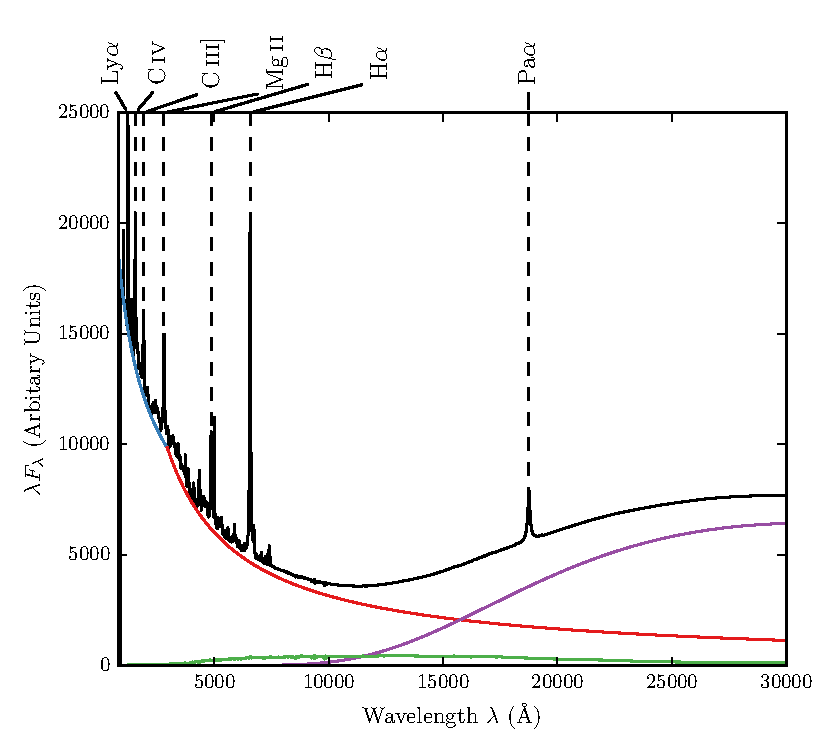
\includegraphics[width=\textwidth]{figures/chapter06/sed_model.pdf}
  \caption{Model spectrum at $z=1$, showing the contributions to the total flux from the blue power-law slope, red power-law slope, blackbody and host galaxy. The locations of the most prominent emission lines in the spectrum are also indicated. }
  \label{fig:modelsed}
\end{figure}

I have constructed a new SED model which reproduces the SEDs of AGNs from the rest-frame UV ($\sim 0.1 \mu$m) to the rest-frame near-IR ($\sim 3 \mu$m). 
In this section, I will describe how I have modelled the emission from the various components contributing to the emission in this spectral region. 
The model spectrum is shown in Figure \ref{fig:modelsed}, with each of the main components indicated. 

\subsection{Accretion Disk}

More than half the bolometric luminosity of an unobscured AGN is emitted in the Big Blue Bump, which extends from the near-IR at 1 $\mu$m to past 0.1 $\mu$m in the UV, and possibly all the way to the soft X-ray region.
The Big Blue Bump emission is thought to arise from an accretion disc. 
In the 0.1 - 1 $\mu$m region the spectrum is generally characterised by a power-law of the form $F_\nu = C\nu^{-\alpha}$ where $\alpha$ is the power-law index, $C$ is a constant, and $F_\nu$ is the flux per unit frequency, usually measured in units of erg s$^{-1}$ cm$^{-2}$ Hz$^{-1}$. 
Equivalently this can be expressed as $F_\lambda = C^\prime\lambda^{\alpha - 2}$ where $F_\lambda$ is the flux per unit wavelength, usually measured in units of s$^{-1}$ cm$^{-2}$ \AA$^{-1}$. 

The value of the power-law index is uncertain. 
From a theoretical perspective, models of geometrically thin accretion discs \citep{shakura73} assume, in particular, that the disc is stationary, axisymmetric, and extends down to the innermost stable circular orbit, and that angular momentum is transported by local `viscous' stresses that convert gravitational energy entirely into heat. 
This gives the dependence of the effective temperature on radius as $t_{\rm eff} \propto r^{-3/4}$. 
A spectrum is then calculated by dividing the disc into concentric annuli, calculating the spectrum emitted by each annulus and then summing them all together. 
Assuming that each annulus radiates like a blackbody, the $r^{-3/4}$ effective temperature distribution gives $F_\nu \propto \nu^{1/3}$ \citep{peterson95}, although it is unclear whether this is consistent with observations.    

In our model we characterised the Big Blue Bump from $\sim 0.1 - 1 \mu$m as a broken power-law with three free parameters: a break-wavelength $\lambda_{\rm break}$, a blue power-law index $\alpha_{\rm blue}$ for wavelengths shorter than the break wavelength, and a red power-law index $\alpha_{\rm red}$ for wavelengths longer than the break wavelength.   

\subsection{Hot Dust}

At wavelengths longer than $1\mu$m, emission from hot dust begins to dominate over emission from the accretion disc. 
The SED in this region is generally characterised either by a power-law ($\propto \lambda^{\beta_{\rm NIR}}$), with $\beta \simeq 0.5$ \citep[e.g.][]{richards06, zhang14}, or by a blackbody at $\sim 1300$ K, thus peaking in the near-IR \citep[e.g.][]{leipski14}. 
We modelled the hot dust emission using a simple blackbody:

\begin{eqnarray}  
  F_\lambda =\frac{2 hc^2}{\lambda^5}\frac{1}{ e^{\frac{hc}{\lambda k_\mathrm{B}T}} - 1} 
\end{eqnarray}

The blackbody component has two free parameters: the temperature of the blackbody $T_{\rm BB}$ and the overall normalisation. 
 
\subsection{Emission Lines}

Hundreds of emission lines are present in a typical AGN spectra. 
Some of the most prominent lines are shown in Figure \ref{fig:modelsed}. 
The emission line spectrum is taken from \citet{maddox06}, who extend the composite of \citet{francis91} to include the H$\alpha$ (6560\AA) and Pa$\alpha$ (18750\AA) emission lines. 
A single parameter, EL$_{\rm scale}$, scales the equivalent widths of all emission lines equally:

\begin{eqnarray}
  F_{\lambda} =  {\rm EL}_{\rm scale} \times \frac{F_{\lambda, \rm el}}{F_{\lambda, \rm cont}} \times F_{\lambda} 
\end{eqnarray} 

where $F_{\lambda, \rm el}$ is the line flux in the template, $F_{\lambda,\rm cont}$ is the continuum flux in the template, and $F_{\lambda}$ is the continuum flux in the model.  

\subsection{Host Galaxy}

Emission from the host galaxy is important, particularly in the region around the $1\mu$m inflection point in the quasar SED. 
While the host galaxies of bright quasars tend to be massive, bright ellipticals, the hosts of lower luminosity AGN can have disc components \citep[e.g.][]{dunlop03}. 
Our model incorporates $z=0$ Sa, Sb, Sc and elliptical-type templates from \citet{mannucci01}, which for simplicity do not evolve with redshift. 
We characterise the relationship between the luminosity of the AGN $L_{\rm AGN}$ and the luminosity of the host galaxy $L_{\rm Gal}$ as a power-law

\begin{eqnarray}
  \label{eq:lgal}
  L_{\rm Gal} = L_{\rm AGN}^{\beta} 
\end{eqnarray}

with power-law index $\beta=0.42$ \citep{maddox06}. 
Dividing both sides of Equations \ref{eq:lgal} by the luminosity of the AGN gives the luminosity of the host galaxy relative to the luminosity of the AGN

\begin{eqnarray}
  \frac{L_{\rm Gal}}{L_{\rm AGN}} = L_{\rm AGN}^{\beta - 1} 
\end{eqnarray}

which for $\beta < 1$ decreases with increasing AGN luminosity. 
In a flux limited sample, the AGN luminosity will tend to increase with redshift and so the luminosity of the host galaxy relative to the luminosity of the quasar will decrease with increasing redshift. 
Hence, the contribution from the host galaxy to the total flux is important at low redshift, but becomes gradually less significant towards higher redshifts. 

Since the contribution from the host galaxy to the flux changes as a function of AGN luminosity, and hence redshift, we choose a reference redshift $z_{\rm nrm}$ where we set the fractional contribution of the host galaxy to the total flux, $\eta$. 
In an arbitrary region of the spectrum (we use $4000 - 5000$ \AA) we calculate both the AGN continuum flux $F_{\rm AGN}(z_{\rm nrm})$ and the flux from our host galaxy template spectrum $F_{\rm Gal}(z_{\rm nrm})$. 
The fractional contribution from the host galaxy to the total flux is then:

\begin{eqnarray}
  \label{eq:eta}
  \eta = \frac{CF_{\rm Gal}(z_{\rm nrm})}{F_{\rm AGN}(z_{\rm nrm}) + CF_{\rm Gal}(z_{\rm nrm})}
\end{eqnarray}

where the constant $C$ is the factor by which we must multiply the unnormalised galaxy spectrum in order for Equation \ref{eq:eta} to hold true. 
Rearranging for the constant $C$ we find

\begin{eqnarray}
  C = \frac{\eta}{1 - \eta} \frac{F_{\rm AGN}(z_{\rm nrm})}{F_{\rm Gal}(z_{\rm nrm})}
\end{eqnarray}
 
Hence at redshift $z_{\rm nrm}$ the host galaxy flux we add to our rest frame quasar continuum is 

\begin{eqnarray}
  \label{eq:flambda}
  F_{\lambda} = \frac{\eta}{1 - \eta} \frac{F_{\rm AGN}(z_{\rm nrm})}{F_{\rm Gal}(z_{\rm nrm})} F_{\lambda,{\rm Gal}}
\end{eqnarray}

where $F_{\lambda,{\rm Gal}}$ is our host galaxy template spectrum in the quasar rest frame. 
The contribution from the host galaxy at a different redshift $z$ is given by  

\begin{eqnarray}
  F_{\lambda} & = & \frac{\eta}{1 - \eta} \frac{F_{\rm AGN}(z)}{F_{\rm Gal}(z)} \frac{F_{\rm AGN}(z_{\rm nrm})}{F_{\rm Gal}(z_{\rm nrm})} \left( \frac{F_{\rm AGN}(z)}{F_{\rm Gal}(z)} \right)^{-1}  F_{\lambda,{\rm Gal}} \\ 
& = &  \frac{\eta}{1 - \eta} \frac{F_{\rm AGN}(z)}{F_{\rm Gal}(z)} \frac{F_{\rm AGN}(z_{\rm nrm})}{F_{\rm Gal}(z_{\rm nrm})}  \frac{F_{\rm Gal}(z)}{F_{\rm AGN}(z)}   F_{\lambda,{\rm Gal}} \\ & = &  \frac{\eta}{1 - \eta} \frac{F_{\rm AGN}(z)}{F_{\rm Gal}(z)} \frac{L_{\rm AGN}(z_{\rm nrm})}{L_{\rm Gal}(z_{\rm nrm})}  \frac{L_{\rm Gal}(z)}{L_{\rm AGN}(z)}  F_{\lambda,{\rm Gal}}  \\ & = & \frac{\eta}{1 - \eta} \frac{F_{\rm AGN}(z)}{F_{\rm Gal}(z)} \frac{L_{\rm AGN}(z_{\rm nrm})}{L_{\rm AGN}(z_{\rm nrm})^\beta}  \frac{L_{\rm AGN}(z)^\beta}{L_{\rm AGN}(z)}  F_{\lambda,{\rm Gal}} \\ & = &  \frac{\eta}{1 - \eta} \frac{F_{\rm AGN}(z)}{F_{\rm Gal}(z)} \left( \frac{L_{\rm AGN}(z)}{L_{\rm AGN}(z_{\rm nrm})} \right)^{\beta - 1}  F_{\lambda,{\rm Gal}}
\end{eqnarray}

We need to know how the luminosity of the AGN depends on redshift. 
This is given by:

\begin{eqnarray}
  \frac{L_{\rm AGN}(z)}{L_{\rm AGN}(z_{\rm nrm})} = 10^{-0.4(M_{\rm AGN}(z)-M_{\rm AGN}(z_{\rm nrm}))}
\end{eqnarray}

where $M_{\rm AGN}(z)$, the absolute magnitude of an AGN at redshift $z$, is given by

\begin{eqnarray}
  M(z) = m - 5({\rm log_{10}}D_{\rm L}(z) - 1)
\end{eqnarray}

and $D_{\rm L}(z)$ is the luminosity distance to a source at redshift $z$ in parsecs. 
Hence:

\begin{eqnarray}
  \frac{L_{\rm AGN}(z)}{L_{\rm AGN}(z_{\rm nrm})} & = & 10^{-0.4(M_{\rm AGN}(z)-M_{\rm AGN}(z_{\rm nrm}))} \\
  & = & 10^{({\rm log_{10}} \left( \frac{D_{\rm L}(z)}{D_{\rm L}(z_{\rm nrm})} \right)^2 )}
\end{eqnarray}

\subsection{Lyman-$\alpha$ Forest Absorption}
\todo{As Paul how he implements this. My code for this can easily be sped up.}

The optical spectra of high redshift quasars show hundreds of sharp absorption lines, which mostly correspond to the redshifted neutral hydrogen Ly$\alpha$ 1216\AA~transition. 
These absorption features are collectively referred to as the {\it Lyman-$\alpha$ forest}. 
To simulate the effect of Lyman-$\alpha$ forest absorption on our model SED we use the parametrisation of \citet{becker13}, who derived an analytic function for the effective optical depth $\tau_{\rm eff}$ over the redshift range 2 $< z <$ 5 made using 6065 quasar spectra from SDSS DR7. 
In their model the effective optical depth $\tau_{\rm eff}$ is given by 

\begin{eqnarray}
  \label{eq:taueff}
  \tau_{\rm eff} & = & \tau_0 \times ( \left( \frac{ 1 + z }{ 1 + z_0 } \right)^b + C )
\end{eqnarray}

where,

\begin{eqnarray*}
  t_0 & = & 0.751 \\
  b & = & 2.9 \\
  C & = & -0.132 \\
  z_0 & = & 3.5 
\end{eqnarray*}

The transmitted flux $F_{\lambda,{\rm trans}}$ at redshift $z$ is then given by 

\begin{eqnarray}
  \label{eq:ftrans}
  f_{\lambda,{\rm trans}} = F_\lambda \times e^{ -\tau_{\rm eff} }
\end{eqnarray}

An absorption line at $\lambda_{\rm abs}$ in the rest-frame of an AGN at redshift $z_{\rm AGN}$ has wavelength 

\begin{eqnarray}
  (1 + z_{\rm AGN})\lambda_{\rm abs} 
\end{eqnarray}

in the rest frame of an observer on Earth. 
In the rest-frame of a cloud of neutral hydrogen at redshift $z_{\rm cloud}$ the absorption line has wavelength 

\begin{eqnarray}
  \frac{ (1 + z_{\rm AGN}) \lambda_{\rm abs} } { (1 + z_{\rm cloud}) }
\end{eqnarray}

and so to absorb Lyman-$\alpha$ at 1216 \AA~ the gas cloud must be at a redshift

\begin{eqnarray}
  \label{eq:zcloud}
  z_{\rm cloud} = \frac{ (1 + z_{\rm AGN}) \lambda_{\rm abs} } { 1216{\rm \AA} } - 1
\end{eqnarray}

For every wavelength $\lambda_{\rm abs} < 1216$ \AA~ in the rest-frame of an AGN at redshift $z > 2$ we calculate $z_{\rm cloud}$ using Equation \ref{eq:zcloud} and then calculate the transmitted flux at $\lambda_{\rm abs}$ by substituting $z_{\rm cloud}$ in to Equations \ref{eq:taueff} and \ref{eq:ftrans}. 

\subsection{Lyman-Limit Systems}

\todo{Ask Paul if this should be implemented}
{\it Lyman-limit systems} are clouds of HI which are optically thick at the Lyman limit ($912$\AA), which generally implies a neutral hydrogen column density $N(HI) > 10^{17} {\rm cm}^{-2}$. 
Photons at wavelengths shorter than the Lyman-limit will be absorbed, which creates a sharp break in the observed continuum. 
We model the effect of a Lyman-limit system at the redshift of the quasar by setting the flux at wavelengths less that 912\AA~ in the quasar rest frame to zero.   

\subsection{Dust Extinction} 

The selection criteria of the SDSS DR7Q catalogue, and particularly the DR10Q catalogue, are sensitive to quasars with moderate amounts of dust reddening \citep[possibly as high as E(B-V) $\sim$ 0.5;][]{richards03} at the redshift of the quasar, and so we included the effect of dust extinction in our model. 
We considered four types of extinction curve: the Large Magellanic Cloud (LMC), Small Magellanic Cloud (SMC), Milky-Way (MW) extinction curves from \citet{pei92} and an extinction curve appropriate for the quasar population which has been derived by Paul Hewett. 
To derive the quasar extinction curve, UKIDSS photometry was used to provide an E(B-V) estimate, via the magnitude displacement of each quasar from the locus of unreddened objects. 
At redshifts $2 < z < 3$ the reddening measure is made at rest-frame wavelengths 3500-7000\AA, where Galaxy, LMC and SMC extinction curves are very similar. 
The SDSS spectra of the same objects are then employed to generate an empirical extinction curve in the ultraviolet, down to 1200\AA. 
The resulting curve has no 2200\AA~ feature and rises rapidly with decreasing wavelength but is not as steep as the SMC curve. 
The extinctions curves give the colour excess $E(B-\lambda)$ relative to the colour excess $E(B-V)$ as a function of wavelength $\lambda$. 
The colour excess $E(B-V)$ is related to the extinction in the $V$ band, $A(V)$, via a parameter $R$, 

\begin{eqnarray}
  A(V) = R \times E(B -V )
\end{eqnarray}

where $R = 3.1$ in the MW and $R \simeq 3$ in the Magellanic Clouds. 
Hence the extinction at a wavelength lambda $A(\lambda)$ is 

\begin{eqnarray}
  A(\lambda) = E(B-V) \times \left[ \frac{E(\lambda-V)}{E(B-V)} + R \right] 
\end{eqnarray}

where the colour excess $E(B-V)$ is a free parameter in our model. 
The attenuation of the flux at a given wavelength is then:

\begin{eqnarray}
  F_\lambda = F_\lambda10^{-A(\lambda)/2.5}
\end{eqnarray}

in the rest frame of the quasar. 

\section{The `Standard' SED Model} 

We will begin by deriving a `standard' SED model by constraining a single set of parameters with a large sample of $0.2 < z < 4$ quasars encompassing a range of luminosities, accretion rates etc. 
The free parameters in our model are the blue power-law slope, the red power-law slope, the power-law break wavelength, the blackbody temperature, the blackbody normalisation, the emission line equivalent width scaling, and the fractional contribution from the host galaxy to the total flux. 
The reddening E(B-V) is fixed to zero, since a large fraction of SDSS quasars have very small amounts of dust reddening \citep{richards03}. 
For the host galaxy we use a Sb-type template derived by \citet{mannucci01}. 
With some choice of initial parameters, we generate a set of model observed spectra at redshifts from $z=0.25$ to $z=3.75$ in intervals of $\Delta z = 0.1$. 
We then transform our set of model spectra into a set of model $ugrizYJHKW1W2$ SEDs 

\begin{figure}
  \centering
  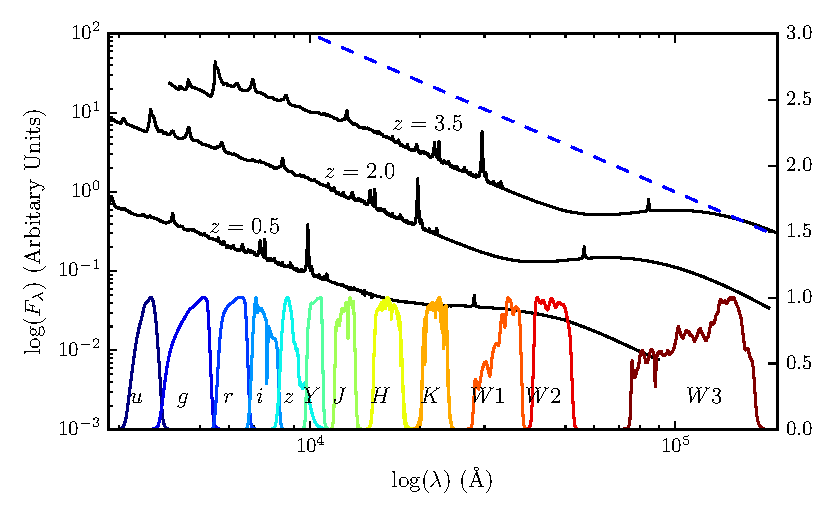
\includegraphics[width=\textwidth]{figures/chapter06/throughput.pdf}
  \caption{Model spectrum at three different redshifts (each arbitrarily scaled), and throughput functions for SDSS, UKIDSS and WISE band-passes (scaled so that the peak transmission is equal to one.) The dashed line indicates the slope of the AB magnitude system zero point.}
  \label{fig:filters}
\end{figure}

The throughput functions of the SDSS $ugriz$, UKIDSS $YJHK$ and WISE $W1W2W3$ band-passes are shown in Figure \ref{fig:filters}, along with our model AGN spectra at three different redshifts. 
The mean flux density in a band-pass P is given by 

\begin{eqnarray}
  \label{eq:flux}
  f_{\lambda}(P) & = & \frac{\int P(\lambda) f_\lambda(\lambda) \lambda d\lambda }{\int P(\lambda) \lambda d\lambda}
\end{eqnarray}

where $P(\lambda)$ is the dimensionless throughput function of the band-pass. 
The corresponding magnitude, $m_\lambda(P)$, is then 

\begin{eqnarray}
  m_\lambda(P) & = & -2.5{\rm log}(f_\lambda(P)) - m_0(P)
\end{eqnarray}

where $m_0(P)$ is the zero-point magnitude of band $P$. In the AB magnitude system, the zero-point flux per unit wavelength is 

\begin{eqnarray}
  \frac{f_\lambda(\lambda)}{{\rm erg}~{\rm cm}^{-2}~{\rm s}^{-1} {\rm\AA}^{-1}} = 0.1087 \left(\frac{\lambda}{\rm \AA}\right)^{-2} .
\end{eqnarray}

This is substituted into Equation \ref{eq:flux} to give a zero-point mean flux density which is then converted into a corresponding magnitude.  

The model SEDs are normalised such that the $i$ magnitude of each model SED is 18.0 mag. 
This gives us an array of model magnitudes as a function of redshift and band-pass. 
We generate an equivalent data array by dividing our quasar sample into redshift bins from $z=0.2$ to $z=3.8$ with bin width $\Delta z = 0.1$. 
We normalise the individual quasar SEDs such that the observed $i$ magnitude is equal to 18.0 mag, and then calculate a median SED in each redshift bin. 

To fit the model to the data we minimise the sum of the squares of the differences between the elements in the model magnitude array and the elements in the data magnitude array. 
The minimisation is done using the `nelder-mead' algorithm. 
Our SED model is valid only up to $\lambda \sim 3\mu$m in the quasar rest frame (the approximate wavelength of the peak in hot dust emission); beyond this additional contributions to the total flux from cooler dust will become significant. 
This prevents us from using the two highest wavelength WISE bands in the fit. 
We also exclude the SDSS $u$ and $g$ band-passes from the fit at $z > 2.7$ and $z > 3.7$ respectively, where absorption in the Lyman$\alpha$ forest becomes large. 

The best-fitting parameters from the fit are shown in Table \ref{tab:params}. 
\todo{Re-do fit}
The colours ($u - g$, $g - r$, etc.) of the median SED, the individual quasars, and the best-fitting model are plotted as a function of redshift in Figs.~\ref{fig:color_1} and \ref{fig:color_2}.  
Most of the large variations that can be seen in the median colours of the quasars as a function of redshift are due to strong emission lines being redshifted in to and out of the bandpasses of the band-passes being used. 

\begin{table}
  \centering
  \begin{tabular}{c c c c}
    \hline 
    Parameter & Symbol & Before Correction & After Correction \\
    \hline 
    Blue power-law index & $\alpha_{\rm blue}$ & 0.58 & 0.58 \\
    Red power-law index & $\alpha_{\rm red}$ & -0.04 & -0.05 \\
    Power-law break & $\lambda_{\rm break}$ & 2945 & 2957 \\
    Blackbody temperature & $T_{\rm BB}$ & 1216 K & 1186 K \\
    Blackbody normalisation & $C_{\rm BB}$ & 0.22 & 0.21 \\
    Emission line scaling & $C_{\rm EL}$  & 0.63 &  0.73 \\
    Galaxy fraction & $\eta$ & 0.29 & 0.28 \\
    E(B-V) & E(B-V) & 0.00 & 0.00 \\
    \hline
  \end{tabular}
  \caption{Best-fitting parameters from fit to DR7Q-matched sample. \todoinline{Only give best-fit values after correction.}}
  \label{tab:params}
\end{table}

\begin{figure}
\makebox[\textwidth][c]{
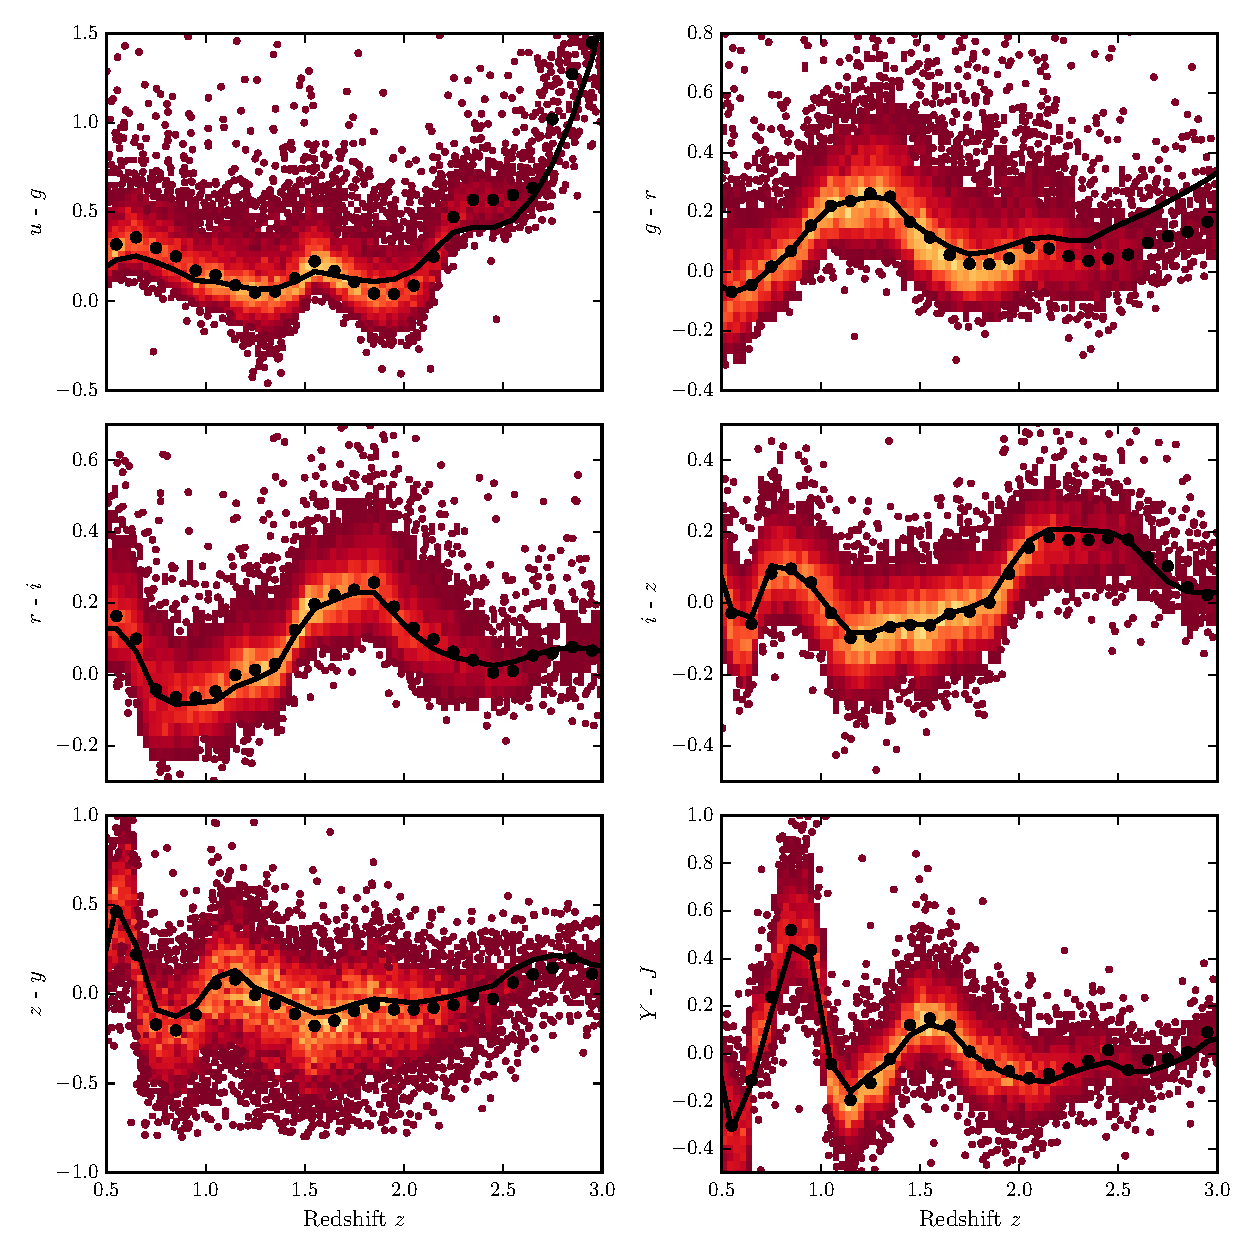
\includegraphics[width=1.3\textwidth]{figures/chapter06/sed_color_plot_1.pdf}
}
\caption{Colours of median SED ({\it black circles}), individual objects ({\it grey points}), best-fitting  model ({\it black line}) as a function of redshift.}
  \label{fig:color_1}
\end{figure} 


\begin{figure}
\makebox[\textwidth][c]{
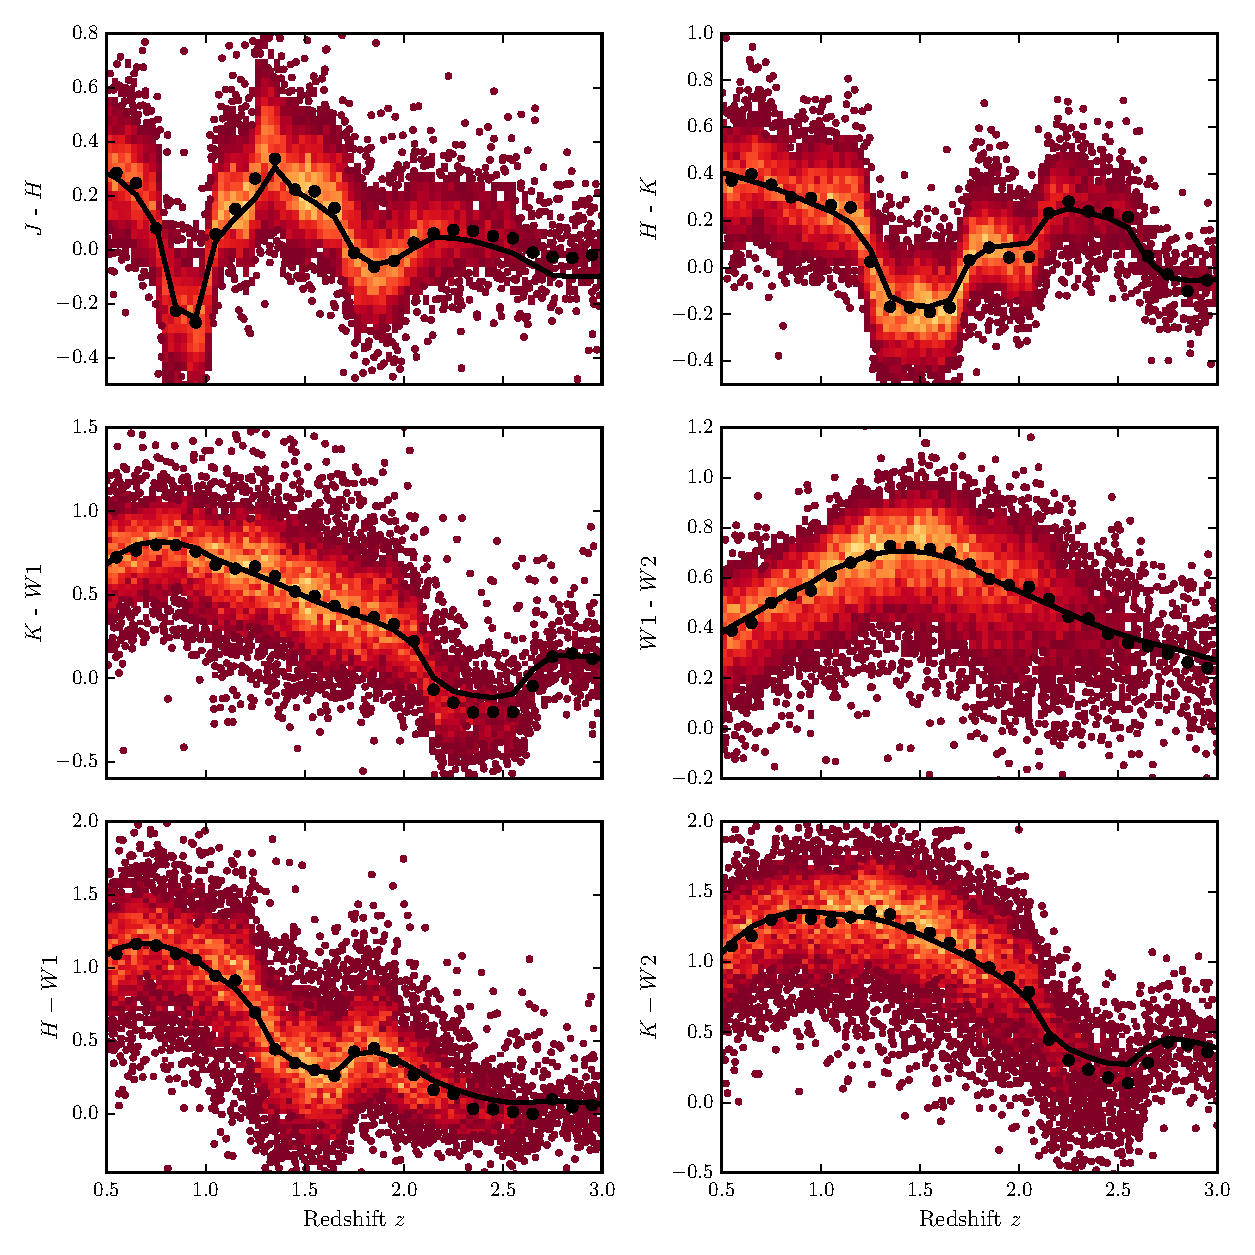
\includegraphics[width=1.3\textwidth]{figures/chapter06/sed_color_plot_2.pdf}
}
\caption{Colours of median SED ({\it black circles}), individual objects ({\it grey points}), best-fitting  model ({\it black line}) as a function of redshift.}
  \label{fig:color_2}
\end{figure} 

\section{Discussion of Fit}

\begin{figure}
  \centering
  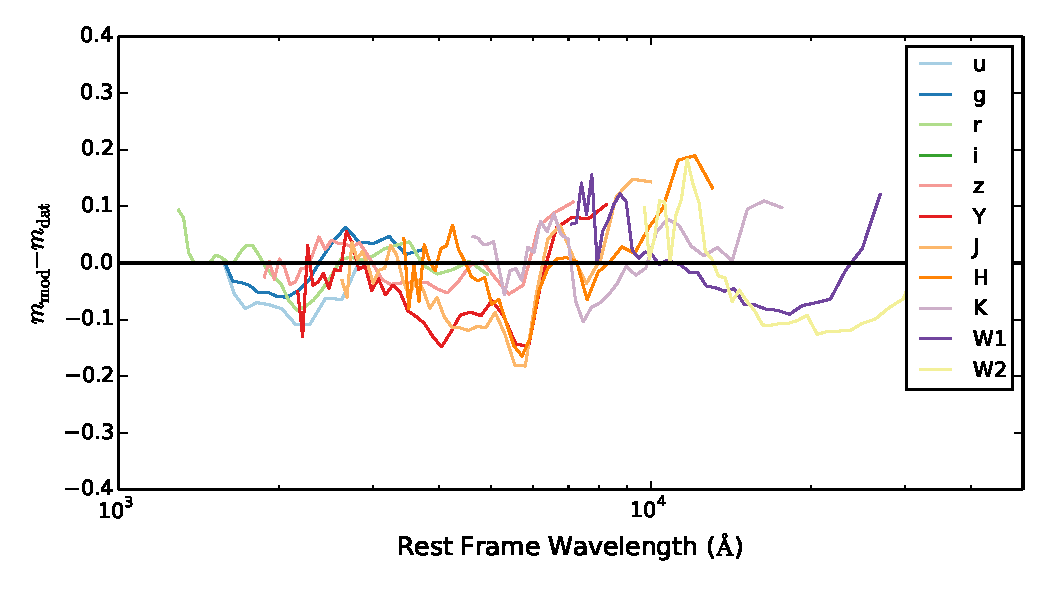
\includegraphics[width=\textwidth]{figures/chapter06/residuals_nocorr}
  \caption{Residuals from fit to DR7Q-matched catalogue as a function of rest-frame wavelength.}
  \label{fig:residuals}
\end{figure}

In Figure \ref{fig:residuals} we show the difference between the magnitudes from the best-fitting model and the median magnitudes from the sample. 
We have transformed the effective wavelengths of the band-passes to the rest frame of the quasars in each redshift bin, to give to the residuals as a function of rest-frame wavelength. 
We represent the residuals measured in each band-pass using a different coloured line. 
Differences between residuals from different band-passes at the same rest-frame wavelength could indicate redshift evolution of the typical quasar SED. 

The residuals indicate that over a large redshift range the model does a fairly good at reproducing the median observed colours of the DR7Q-matched sample. 
Most discrepancies are at the $<0.1$ mag level. 
It is remarkable that a single model is so effective; the properties of a typical quasar to not change significantly over a wide range of redshifts and luminosities. 
On the other hand, for the individual objects there is a significant scatter about the mean. 
In general, our goal is to use this intrinsic spread in SED properties in order to understand the diversity in physical quasar properties. 

\subsection{Flux Correction}

\todo{I have text on empirical correction. Re-do once I am happy with SED model}
% The most noticeable feature in Figure \ref{fig:residuals} is a bump around 1$\mu$m, where the model underestimates the flux of the population by $\sim 0.1$ mag. 
% If the model is a poor fit to the data, it can produce strong redshift-dependent systematics. 
% A blackbody component with a higher temperature would contribute more flux in this region, which could potentially lead to redshift-dependent systemetatic errors. 
% To avoid this we derived a correction to our model which accounted for the $1 \mu$m flux discrepency. 

% We fit the overall normalisation of the model SED only; this is a constant vertical displacement we add to the model magnitudes. 
% This fit is done in the 2000 - 9000 \AA~ region of the rest frame spectrum using our sample of `standard' quasars. We calculate the $m_{\rm data} - m_{\rm model}$ residuals for each quasar, and calculate the effective wavelength of each band-pass in the rest frame of the quasar. 
% In Figure \ref{fig:modelcorrection} we show a 101-point running median through the residuals of each band-pass in the 6000 - 22000 \AA~ region of the quasar rest frame. 
% The lines have been colour-coded to show the redshifts of the quasars which are contributing to the residuals in the corresponding region of the quasar rest frame. 
% The black line in the Figure \ref{fig:modelcorrection} is a cubic interpolation of a 801-point running-median through all residuals as a function of the quasar rest frame wavelength, irrespective of the band-pass used. 
% It shows quite clearly that the model is underestimating the observed flux over the $\sim 8,000 - 17,000$\AA~ rest frame wavelength region. 
% We calculated the multiplicative factor which when applied to the model spectrum accounted for the model to data magnitude discrepancy, i.e. the amount of flux `missing' from the model. 
% In the bottom panel of Figure \ref{fig:modelcorrection} we show our model spectrum both with and without this correction term. 
% In Figure \ref{fig:colorplots} we show how the fit is imporved in the $\sim 1\mu$m region of the rest frame spectrum. 

% \begin{figure}
%   \centering
%   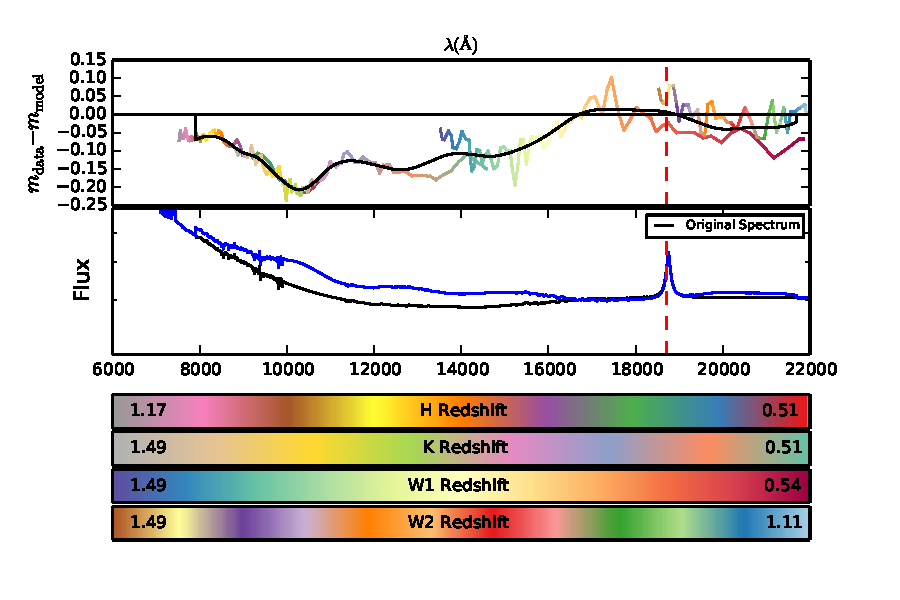
\includegraphics[width=\textwidth]{figures/chapter06/residualscorrection}
%   \caption{{\it Top:} Residuals from fitting the overall normalisation of the SED as a function of wavelength in the quasar rest frame. The different lines correspond to 101-point running medians for the $H$, $K$, $W1$ and $W2$ band-passes, and have been colour-coded to indicate the redshift for which the given quasar rest frame wavelength corresponds to the un-redshifted effective wavelength of the band-pass. The black line is a cubic interpolation of a 801-point running-median through through all residuals, irrespective of the band-pass used. The red dashed line marks the wavelength of the Pa$\alpha$ emission line. {\it Bottom:} The spectral model before and after the flux correction ({\it see main text}).}
%   \label{fig:modelcorrection}
% \end{figure}

% Later on in Section \ref{sec:fluxcorrection} we will derive an empirical correction to the model which increases the flux slightly in the 8000 to 17000 \AA~ region of the rest frame spectrum. 
% The red lines in Figure \ref{fig:colorplots} show the colours of this corrected model as a function of redshift. Although the correction improves the fit slightly, significant discrepancies do remain. 
% The model's underestimation of the flux at in the 3$\mu$m region is probably due to the increasingly significant contribution to the flux from cooler dust at longer wavelengths, which is not included in our model. 
% We will discuss this in more detail in Section \ref{sec:definingsample}. 

% Our fitting scheme scales the equivalent width of every emission line by the same amount. 
% Observationally, the emission line ratios are not the same for every quasar, and the model to data discrepancies in certain regions are likely to be the result of this. 
% In Figure \ref{fig:residuals} we mark the position of the \ha emission line, which is typically very strong and broad and can contribute significantly to the flux even in a broad band-pass. 
% The relatively large residuals around the wavelength of the \ha line may suggest that our simple scaling scheme is insufficient, and we may need to allow the equivalent widths of certain prominent emission lines to vary freely. 

\section{Hot Dust}

Above we have shown that, with a single parametric model, we are able to very accurately match the average colours of quasars over an enormous range in redshift ($0.2 < z < 4$) and luminosity ($10^44 < L_Bol < 10^48$\ergs). 
Below, we will focus on a a sample of unreddened quasars, concentrating on redshifts 1.0-1.5 (where we have full rest-frame coverage to 2 microns) and low galaxy contribution, with a view to looking at the redshift 2.0-2.7 range where we do have the \ion{C}{IV} and other UV-spectrum information. 
Our main result is linking the instrinsic spread in the near-IR SED to properties of the AGN.

\subsection{Introduction}

Significant diversity in quasar SEDs is observed, the most obvious difference being the Type I/II dichotomy, which is explained by orientation-based unification schemes (Antonucci 1993). 
Such schemes require an anisotropic parsec scale obscuring structure that surrounds the central accreting black hole (e.g., Krolik \& Begelman 1988; Antonucci 1993). 
In this picture, the bulk of the radiation from the central engine is absorbed by the obscuring structure (commonly referred to as the torus) and re-emitted mainly in mid-infrared (MIR) wavelengths. 

At the same time, AGN-driven outflows are present in a large fraction of the luminous quasar population. 
The mass and energy associated with these outflows is believed to be significant in the context of feedback and its effect on the host galaxy. 

While orientation-based models, including a parsec-scale obscuring structure, have been successful in explaining some of the diverse properties of quasars (most notably the difference between type 1 and type 2 quasars), quasars are also likely to evolve through fuelling phases. 
Numerical simulations indicate that feedback is triggered in a fueling phase during a gas-rich galaxy merger (Hopkins et al. 2008; Narayanan et al. 2010), satellite accretion or secular processes (e.g. Fanidakis et al. 2012). 
Objects in the early feedback phase are likely to be both highly luminous (accreting close to the Eddington limit) and highly obscured by dusty inflowing material (Haas et al. 2003). 
In time, the energy output of the  central engine becomes sufficiently powerful to drive outflows, which can blow away the obscuring clouds of dust and gas. 
The quasar emission is then relatively unobscured until it declines as a result of the depletion of the available gas reservoirs. 
As the quasar transitions through these stages in its lifetime, key observational properties, such as the luminosity and the SED, are likely to change. 
Quantitatively, however, it remains unclear how these phases relate to the fundamental properties of the accreting black-hole (e.g.  mass (M$_{\rm{BH}}$), bolometric luminosity (L$_{\rm{bol}}$) and Eddington ratio (L/L$_{\rm{Edd}}$) and the elements of the non-spherical geometry). 
However, multiple authors have found no significant dependence of the spectral energy distribution (SED) on properties such as redshift, bolometric luminosity, SMBH mass, or accretion rate (e.g. Elvis et al. 2012, Hao et al. 2013) and quasars up to redshift 7 have been shown to have similar UV spectra to low redshift quasars (e.g. Mortlock et al. 2011). 

Reverberation measurements of nearby AGNs suggest that the near-infrared (NIR) emission in these sources is dominated by thermal radiation from hot (T$\sim$1200K) dust very close to the central source (few tens of light days; e.g. Minezaki et al. 2004; Suganuma et al. 2006). 
This is the approximate location of the inner-most edge of the dusty torus. 
Previous studies have fitted the NIR–MIR spectral energy distributions (SEDs) of AGNs using a blackbody spectrum to represent emission from hot dust in the inner region of the torus (e.g. Mor et al. 2009; Deo et al. 2011). 
The modelled temperature of this component is high ($\sim$1200 K), and is consistent with pure-graphite dust emission.  
It is not clear that such emission can be consistent with torus emission, which is from cooler dust, which presumably exists further from the nucleus, and peaks at longer wavelengths.  
The conclusion is that the hot dust may be a separate component from the torus dust. 
Several studies have shown that the luminosity of the NIR excess emission correlates with that of the central engine with a slope close to unity (e.g. Gallagher et al. 2007), suggesting that the dust is reprocessing radiation from the accretion disc. 

Outflows may emerge from the outer region of the accretion disc or even the innermost region of the torus, in which the gas clouds are dusty and relatively cold.  
Indeed, there is observational evidence for dusty outflows close to the central engine (e.g. Bowler et a. 2014). The dust is heated by the central engine, and radiates in the near-infrared band. 
Wang et al. 2013, fitting the NIR emission with a single power-law, found that objects with strong outflow signatures (blue-shifted CIV) have more hot dust emission relative to the accretion disc emission in a large sample of $z \sim 2$ non-BAL quasars. 
It could be that this correlation is induced by a third factor that simultaneously affects outflows and dust emission, for instance the inclination angle or metallicity. 
Alternatively the dust could be intrinsic to outflows and may have a non-trivial contribution to the outflow acceleration.

Several studies have identified a population that is missing the hot dust component entirely (Hao et al. 2010, 2011; Jiang et al. 2010; Mor \& Trakhtenbrot 2011). 
The fraction of hot dust poor quasars seems to be a function of redshift, at least at high-redshift. 

With large-scale surveys from SDSS, UKIDSS, and \textit{WISE} providing information on the SEDs covering rest-frame 0.1-3.0\,$\mu$m wavelengths for thousands of AGN at redshifts $2 \lesssim z \lesssim 3$ it is finally possible to study the link between outflow diagnostics from ultra-violet spectra, e.g. as measured from the \ion{C}{IV} emission line, and emission from hot (T $\simeq$ 1200K) dust peaking in the NIR, which provides information about the amount and geometry of gas and dust on parsec scales. 
In one model, quasars are surrounded by an inner `wall' of gas and dust, in a cylinder-like geometry. 
As a radiatively-driven outflow develops, material at the extremes of the cylinder is driven-off, exposing more of the inner edge of the obscuring material at the equator (a `torus'), which contains the hot dust. 
Quasars are also observed with a wide distribution of reddening from dust on galactic scales. 
It is believed that luminous highly dust-reddened quasars may be in the process of expelling their dust and transitioning to ultra-violet bright objects which make up to the majority of the SDSS sample. 
Outflow signatures are very common in the rest-frame optical \ha line profiles of the heavily reddened quasars (Banerji et al. 2012, 2013), but it isn't clear how significant these outflows are on larger, kiloparsec scales.

The WISE photometry provides essentially complete coverage for the SDSS i$<$19.1 quasar sample and the spread in the KW1W2 colours (Figs. 4 \& 5), probing the rest-frame ~1-2 micron region, is significant and strongly suggests presence of real variation in the "hot dust" temperature and luminosity among the quasars. 
Several other investigations have drawn attention to the rest-frame near-infrared SEDs, with populations of "dust free" objects postulated. 

Including a black-body with T$\sim$1250K, matches the ugrizYJHKW1W2 (SDSS+UKIDSS+WISE) median/modal colours for redshifts z=0.2-4.0 extraordinarily well. 
The initial focus has been on a sample of unreddened quasars (Fig. 3), concentrating on redshifts 1.0-1.5 (where we have full rest-frame coverage to 2 microns) and low galaxy contribution, with a view to looking at the redshift 2.0-2.7 range where we do have the CIV and other UV-spectrum information. 
Main result is linking near-IR SED to spectral properties.

With large-scale surveys from SDSS, UKIDSS, and WISE providing information on the SEDs covering rest-frame 0.1-3.0 $\mu$m wavelengths for thousands of AGN at redshifts $2 \lesssim z \lesssim 3$ as well as direct coverage of the rest-frame-UV spectra, it is possible to study the link between outflow diagnostics from ultra-violet spectra and emission from hot dust peaking in the NIR. With our data set we can concurrently infer outflow properties from the SDSS spectra and properties of the NIR emission from the broad-band spectral energy distribution for a large sample of quasars in order to discriminate between different ideas for the structure and kinematics close in the central regions of the quasar. 

The "hot dust" signature could contain information about inner face of whatever form of obscuring torus/disk/... may exist in orientation schemes and/or say something about the dust content in the disk-wind.

One obviously has the information from the SDSS quasar spectrum for all the objects, including "outflow" diagnostics/signatures such as the CIV emission-line profiles.

\subsection{Sample}

Our primary goal is to study the hot dust properties of quasars at redshifts $2 \lesssim z \lesssim 3$, i.e. during the epoch that quasar activity in the Universe peaked. 
In this work, we take advantage of a number of recent, sensitive, wide-field surveys, covering the UV to mid-IR spectral region. 

We include only quasars with observed magnitudes brighter than 19.1 in the $i$ band-pass, i.e. the quasars selected by the main SDSS quasar selection algorithm (70,214 quasars). 
Cross-matching (with a 2$''$ radius and picking only the nearest neighbour) the SDSS DR7Q catalogue with the ULAS catalogue, which covers only $\sim 38$\% of the SDSS foot-print, resulted in 37,886 matches. 
Of these 36,628 have been detected in one or more of the WISE band-passes. 
We exclude quasars flagged as broad-absorption line quasars (BALQSOs; Weymann et al. 1991) from the sample (leaving 35,272 quasars).

We defined two sub-samples: one low-$z$ ($1 < z < 1.5$) and the other high-$z$ ($2 < z < 2.7$). 
As we will demonstrate below, in these two redshift windows we have the best constraints on the hot dust properties of our sample. 
The reason for the lower-bound on the low-$z$ sample is to minimize the contribution from the host galaxy; the relative host galaxy contribution will vary strongly as a function of redshift and quasar luminosity, and so restricting the sample to $z>1$ where the host galaxy contribution is negligible will minimise potential biases in our analysis. 
Constraints on the shape/amount of NIR emission are coming primarily from the K/W1/W2 bands at low-$z$. 
As we will demonstrate in the next section, at $z \gtrsim 1.5$, our ability to constrain the shape of the blackbody component in our SED model is considerably reduced. 
Similar considerations apply to our choice of redshift limits for the high-$z$ sample; these will be expanded upon below. 
We impose a lower-limit signal-to-noise ratio (S/N) $>$ 5 magnitudes in the $K$, $W1$ and $W2$ band-passes for the low-$z$ sample and S/N > 5 in the $W1$, $W2$, and $W3$ band-passes for the high-$z$ sample. 
This gives us 5,910 quasars in our low-$z$ sample and 1,989 quasars in our high-$z$ sample. 
For the high-$z$ sample, the requirement of a S/N > 5 detection in the W3 band removes 25\% of objects. 
We will consider below whether this introduces any bias in to our sample. 

We want to focus on a subset of objects with typical UV/optical emission properties, i.e. typical accretion disc emission, not much dust extinction and no unsually strong broad emission lines. 
We will hold most parameters fixed, and vary only those we are interested in, i.e. the blackbody parameters which parameterise the NIR emission. 
Therefore we need to define a sub-sample of objects which we know are well fit by our standard SED model in the UV/optical region. 
We use the $i-K$ colours of the quasars as a measure of the overall colour of the quasars as it provides the longest baseline in wavelength without being affected by absorption in the Ly$\alpha$ forest at high redshifts. 
To do this we discarded from our sample quasars with $i - K$ colors redder than our standard model with dust reddening E(B-V) = 0.075 and bluer than E(B-V) = -0.075 (see Figure below). 
This region of the $i-K$ colour space includes both quasars with significant amounts of dust redenning and quasars with extreme emission line equivalent widths, or objects with intrinsically very red/blue UV/optical continuum. Obviously negative E(B-V) values are not physical. 
Instead, they arise when the UV/optical continuum is bluer than the power-law slope of our SED model. 
Following this cut we are left with 4,615 quasars in our low-$z$ sample and 1,692 quasars in our high-$z$ sample. 

\begin{figure}
  \centering
  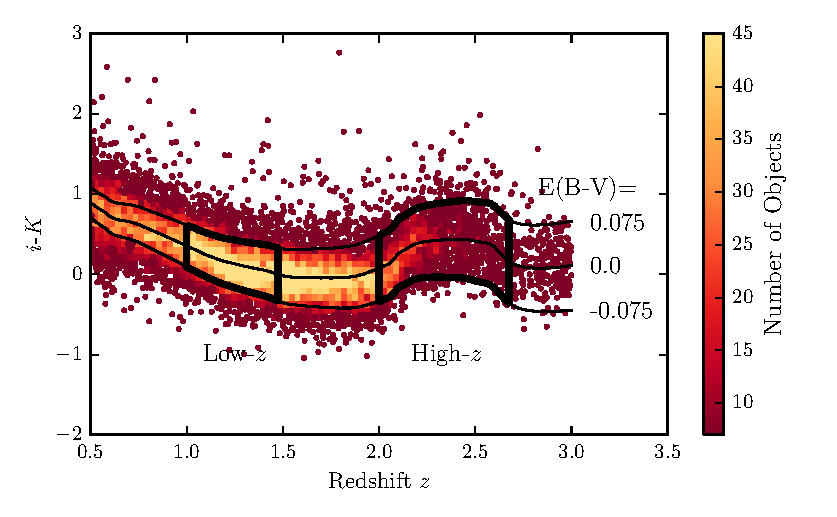
\includegraphics[width=\columnwidth]{figures/chapter06/ik_versus_z_low_ext.pdf}
  \caption{$i-K$ vs $z$. Demonstrates how sample was defined. The grey points show, as a function of redshift, the $i-K$ colours of all DR7Q quasars which are not classified as broad-absorption line quasars by Shen et al. and $i$ magnitude > 19.1. The black line shows the $i-K$ colour of our standard, unreddened SED model as a function of redshift. The red and blue lines show the $i-K$ colours of our SED model with dust reddening E(B-V) = 0.075 and E(B-V) = -0.075 respectively. A significant amount of this reddening can be attributed to intrinsics variations in the UV power-law slopes of the indidual quasars, which is why we allow a negative reddening. However, there is a clear `red tail' to the colour distribution which can be explained by dust reddending at the redshift of the quasar. We definined two samples, at low ($0.5 < z < 1.5$) and high ($2 < z < 2.7$) redshift, which are shown in the figure.}
  \label{fig:ikzplot}
\end{figure}

In Figure~\ref{fig:w1w2colorsratio} we plot the $W1 - W2$ colors of the DR7Q-matched sample as a function of redshift at z < 3. 
In this redshift range the $W1$ and $W2$ band-passes are probing the 1.2 - 2.8$\mu$m and 1.6 - 3.8 $\mu$ region of the rest frame SED respectively. 
For reference, the peak wavelength is at 2.4$\mu$m for a black-body radiating at 1200K (close to the sublimation temperature of dust grains). 
At any given redshift we see a $\sim 0.5$ mag dispersion in the $W1-W2$ colors. 
On the same axes in the Figure we have plotted the $W1 - W2$ colors derived from our SED model with a fixed blackbody temperature (1216K) and a ratio of NIR to UV luminosity ranging from 0.0 to 1.0, with the other model parameters held constant. 
To get the NIR luminosity we integrate the blackbody component of our model. 
To get the UV luminosity we integrate our total model spectrum between 2000 and 9000A.  

\begin{figure}
\centering
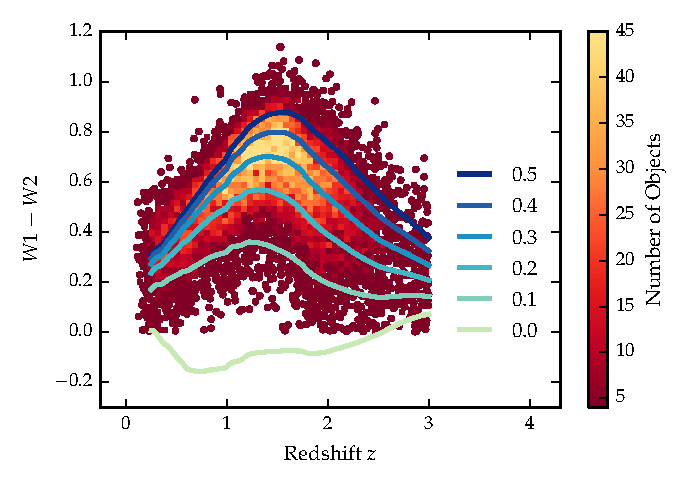
\includegraphics[width=\columnwidth]{figures/chapter06/w1w2_versus_redshift_ratio.pdf}
\caption{$W1 - W2$ colours of DR7 sample as a function of redshift. Above a certain density threshold points are represented by a density plot. On top we plot the colours of our standard SED model, with a fixed temperature and a varying NIR (1 - 3 $\mu$m) to UV ratio. }
  \label{fig:w1w2colorsratio}
\end{figure}

The NIR emission in quasar SEDs is likely due to hot dust at its sublimation temperature, possibly at the inner edge of dusty torus structure. 
We observe that even if we restrict the sample to be fairly uniform in its UV/optical properties, we still get an interesting spread in W1-W2 colors, which we can use to learn about the diversity of NIR properties in our sample. In the rest of this paper we will characterise the hot dust properties of our sample, and test its relation to quasar properties such as luminosity, black-hole mass and normalised accretion rate, and outflow-properties. 
First we will fit single temperature black-bodies to each quasar in our sample, and characterise the distribution of temperatures and luminosities we observe. 
We will begin by describing our fitting procedure. 

\begin{figure}
\centering
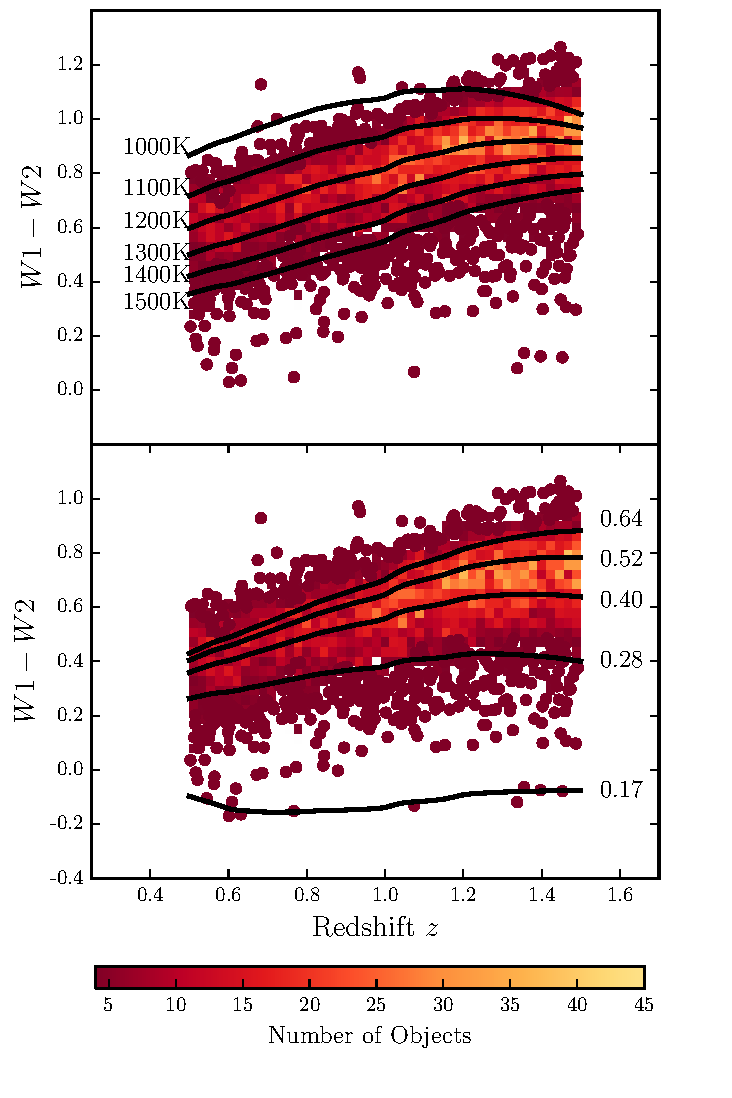
\includegraphics[width=\columnwidth]{figures/chapter06/w1w2_versus_redshift.pdf}
\caption{$W1 - W2$ colours of DR7 sample as a function of redshift, up to $z=1.8$. Above a certain density threshold points are represented by a density plot. On top we plot our standard model, with a blackbody temperature varying from 1000 - 1600 K ({\it top figure}) and a blackbody normalisation between 0 and 0.5 ({\it bottom figure}). Around $z=1.5$ the model no longer appears to be a very good fit to the data, which I suppose is just the fact that the blackbody is turning over, whereas in the data the flux keeps incresing (additional contributions from cooler components.) Add ticks to top of top panel. Think about how useful these plots really are. In top plot I'm changing the temperature, which is changing the normalisation (Lum IR). This is effectively same as bottom plot, except here I'm keeping the shape the same, just moving it up and down. Even if this is fine these plots are probably a bit misleading as they are (need to be clear normalisation will also be changing in the top plot.}
  \label{fig:w1w2colors}
\end{figure}

\section{Fitting procedure}

In this section we need to make clear:
\begin{itemize}
    \item What we are after (hot dust and associated T and L)
    \item What we need by way of rest-frame wavelength to constraint the BB-parameters
    \item How we will then use the available observed-frame passbands, redshift ranges to probe required rest-frame wavelength range
    \item Introduce "tools" for assessing quality of model-SED fits
\end{itemize}

Need (here or earlier) a short discussion on the advantages/disadvantages presented by the fixed observed-frame magnitudes and the quasar redshifts. 
Should include comment on systematics as function of redshift for SED parametrizations that are not perfect as well as increased uncertainty in good parametrizations as redshift change restricts rest-frame wavelength available (e.g earlier should have an "accessible wavelength" and "required-wavelength" to constrain T\_BB discussion). 
One does need to take care in looking at trends with luminosity [in particular] given the observed-frame passband information on the rest-frame SED can produce some strong systematics with redshift, particularly if the SED-model is not a good fit to the actual SED. 
Then introduce "tools" to be used, including simulated SEDs and "residual plots".
 
The initial focus has been on a sample of unreddened quasars (Fig. 3), concentrating on redshifts 1.0-1.5 (where we have full rest-frame coverage to 2 microns) and low galaxy contribution, with a view to looking at the redshift 2.0-2.7 range where we do have the CIV and other UV-spectrum information.

For a given set of parameters, our model returns a flux $F_{\lambda}$ as a function of wavelength (or equivalently frequency) in the UV - NIR region. 
The model spectrum is redshifted to the redshift of the quasar being fit and is then multiplied by the $ugrizYJHMW1W2W3$ throughput functions and normalised appropriately to give AB magnitudes. 
To fit the model to the data we minimise the sum of the squares of the differences between the elements in the model magnitude array and the elements in the data magnitude array. 
The minimisation is done using the 'nelder-mead' method (also known as the downhill simplex method or amoeba method), as implemented in the ${\tt minimize}$ function from the Python module ${\tt scipy}$. 
We characterise the hot dust properties of our sample in terms of the temperature and luminosity of the best-fit black-body. 
We choose to parameterise the luminosity of the hot dust component in terms of the NIR to UV luminosity ratio (which is proportional to the covering factor of hot dust ($L_{NIR}/L_{Bol}$) used in other studies (Roseboom et al. 2013)). 
The UV luminosity is calculated by converting the flux density in to an appropriately normalised luminosity, and then integrating between 2000 and 9000A. 
The NIR luminosity is calculated by converting the black-body flux into a luminosity and then integrating over all wavelengths. 

It's important that we are fitting approximately the same part of the rest frame spectrum of each quasar, to avoid systematic bias with redshift. 
To avoid significant absorption in the Lyman-$\alpha$ forest at high-$z$, we restrict our fitting to wavelengths greater than 2000A; when the effective wavelength of a band-pass falls below this limit the band-pass is excluded from the fit. 
\todo{2000A is quite large given the Lyman-alpha forest impacts from 1216A.}
For our low-$z$ sample, the maximum wavelength being fit is set by the wavelength coverage of the W2 band. 
For our low-$z$ sample, W3 probes rest-frame wavelengths of $\sim 5-6 \mu$m. 
In this wavelength region additional contributions to the total flux from cooler dust at larger radii from the central source will become significant. 
This is obvious in the Figure below, which shows the normalised residuals from our fit. 
As we fit quasars at lower redshifts the discrepancy between the W3 magnitude and the model-predicted W3 magnitudes becomes systematically larger. 
The discrepancy is in the sense that the model is under-predicting the flux we observe; this is very likely due to the fact that our model uses only a single-temperature black-body, and therefore neglects contributions to the SED from cooler dust components (possibly from further out in a dusty torus structure). 
Since we do not attempt to model these components, we exclude information from the W3/W4 bands in our fits. 

Figure below shows how for these fits the two parameters, black-body temperature and luminosity, vary as a function of redshift. 
As we look at higher redshifts, the maximum wavelength in the rest-frame spectrum we are sensitve to is shortened. At z >~ 1.5, the uncertainty in the black-body luminosity increases significantly. 
At z~1.5, W2 is probing ~1.8$\mu$m. 
At higher redshifts our ability to constrain both black-body parameters with the available photometry is diminished. 
This justifies our $z=1.5$ upper limit on our low-$z$ sample.  

Using a similar logic, we have chosen the redshift range of our high-$z$ sample so that W3 is sensitive to the region of the rest-frame spectrum that is dominated by hot dust emission. 
This means a lower-limit of $z=2$; at lower redshifts we see the residuals from the fit begin to increase and systematic changes in the black-body parameters with redshift. 
We set an upper-limit of $z=2.7$ to avoid noise from small number statistics.  

Some care has been taken to ensure that we do not have significant systematics in blackbody temperature (T\_BB) with redshift but we are only attempting to reproduces the $\lesssim3$ micron rest-frame SED. 
Looking to longer wavelengths (with WISE W3) one immediately sees additional flux from dust with lower T\_BB. [Figs 6-10 show small systematics - we aren't intending to reproduce the additional flux at $>$ 3 microns, which is obviously present]. Ignore Fig. 11. 


\begin{figure}
  \centering
  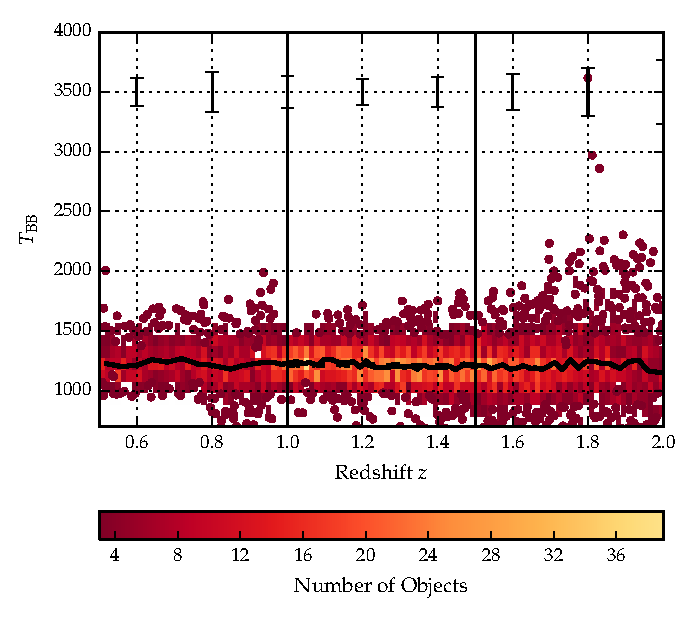
\includegraphics[width=\textwidth]{figures/chapter06/bbt_z_errors.pdf}
  \caption{Black-body temperature as a function of redshift. The errorbars indicate how the mean standard error in the black-body temperature changes with redshift. The solid black line is a 101-point running median which has been smoothed by plotting only one in every 1000 point.}
  \label{fig:}
\end{figure}

\begin{figure}
  \centering
  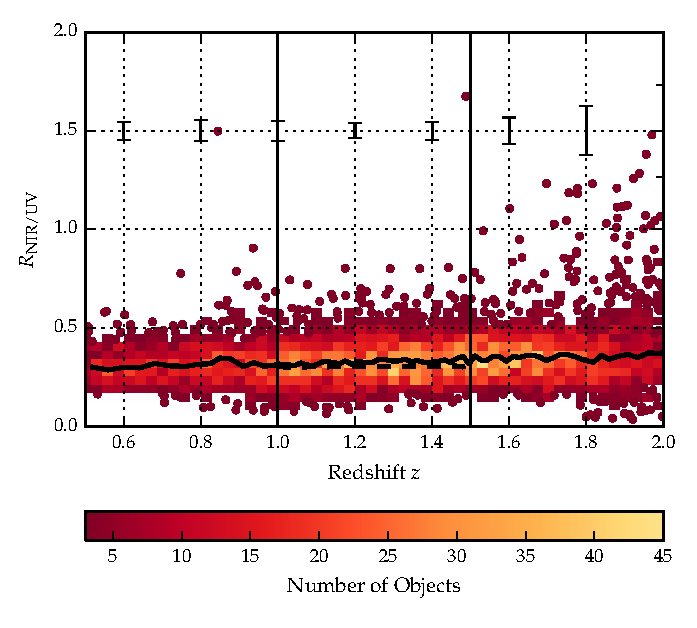
\includegraphics[width=\textwidth]{figures/chapter06/ratio_z_errors.pdf}
  \caption{Ratio of NIR to UV luminosity as a function of redshift. Dashed black line shows how the best-fit parameter changes as we fit a mock data set of SEDs with fixed black-body properties at a range of redshifts.}
  \label{fig:}
\end{figure}

\begin{figure}
  \centering
  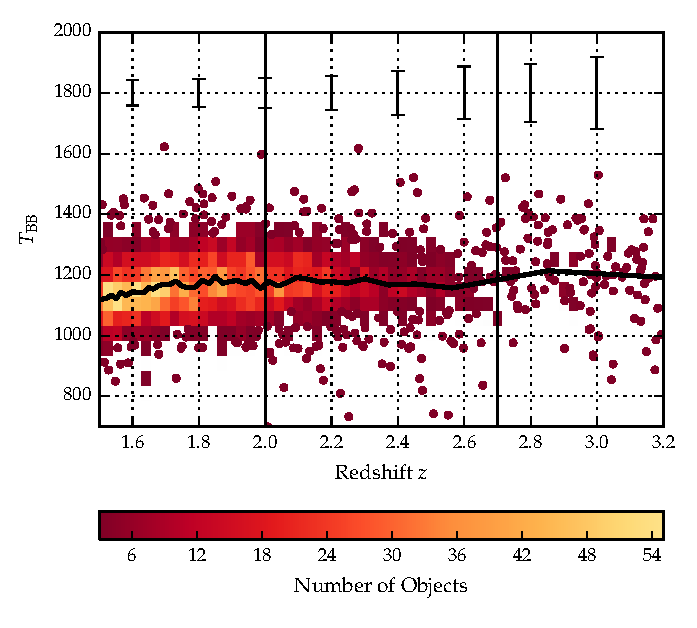
\includegraphics[width=\textwidth]{figures/chapter06/bbt_z_errors_highz.pdf}
  \caption{Black-body temperature as a function of redshift.}
  \label{fig:}
\end{figure}

\begin{figure}
  \centering
  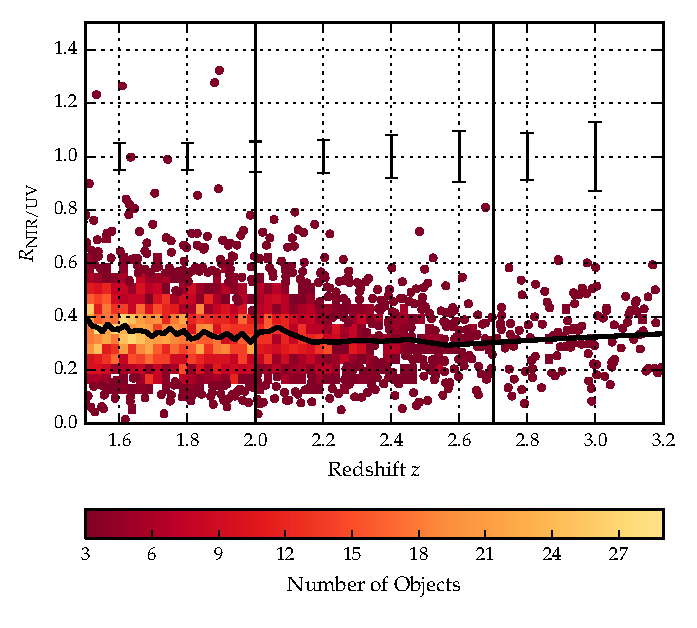
\includegraphics[width=\textwidth]{figures/chapter06/ratio_z_errors_highz.pdf}
  \caption{Ratio of NIR to UV luminosity as a function of redshift.}
  \label{fig:}
\end{figure}


\section{Results}

We want to get all of the caveats out of the way before this section, and in this section present only the results which we believe to be meaningful. 

First we need to understand the degeneracies between the two parameters. 
In Figure~\ref{fig:ratio_tbb_density} we see that the two parameters are clearly correlated. 
For a lower temperature black-body the NIR to UV luminosity ratio is larger. 
Such a correlation is to be expected, as the black-body temperature is lowered, the peak shifts to lower-wavelengths (following Wien's displacement law) where we no longer have any constraints on the hot dust properties (explain more coherently). 
Because of this correlation we need to be very careful to seperate out real trends of $R_{NIR/UV}$ with other quasar properties from indirect trends resulting from a mutual dependence on $T_{BB}$.  

\begin{figure}
  \centering
  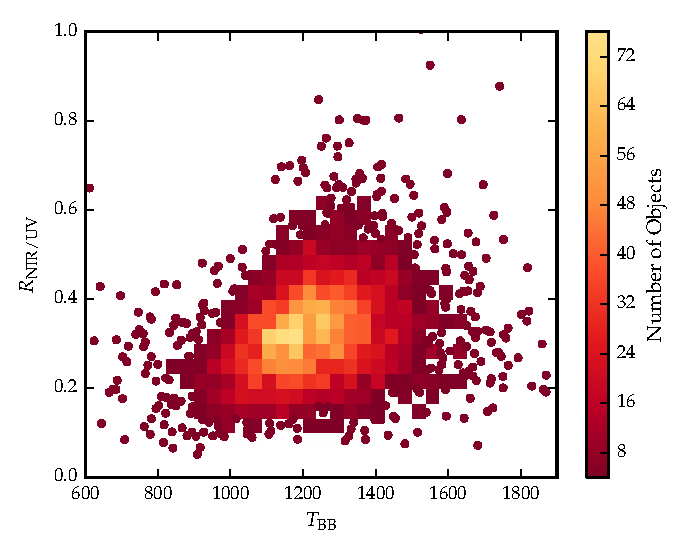
\includegraphics[width=\textwidth]{figures/chapter06/ratio_tbb_density.pdf}
  \caption{Ratio of NIR to UV luminosity ($R_{NIR/UV}$) against temperature ($T_{BB}$) for low-$z$ sample. The density of points is shown in more dense regions of the space, and individual objects in less dense regions. }
  \label{fig:ratio_tbb_density}
\end{figure}

In Figure~\ref{fig:ratio_tbb_density} we show that there is quite a range of temperature and normalisation present in our sample. 
However, we need to check how much of this is due simply to uncertainties in the fits stemming from uncertainties in the photometry. 
In order to achieve this we took our standard SED model with a single temperature and normalisation black-body component, and generated 200 mock SEDs with a brightness distribution similar to that of our real sample. 
We estimated the mean uncertainty of the magnitudes in the K, W1, and W2 band-passes as a function of apparent brightness. 
We then sampled the K, W1, and W2 magnitudes from Gaussian distributions, with a mean equal to the magnitude of the model SED, and the width equal to the mean uncertainty at the appropriate brightness. 
Finally, we fit these mock SEDs using our standard fitting procedure. 
The results are shown in the Figure below, on top of the results from our real sample (shown as grey contours). 
We can see that uncertainty in the photometry introduces a significant scatter to the temperature, but that this scatter is less than the intrinsic scatter in the data. 
This demonstrates that there is a real distribution of hot dust temperatures and luminosities in our sample. 

\begin{figure}
  \centering
  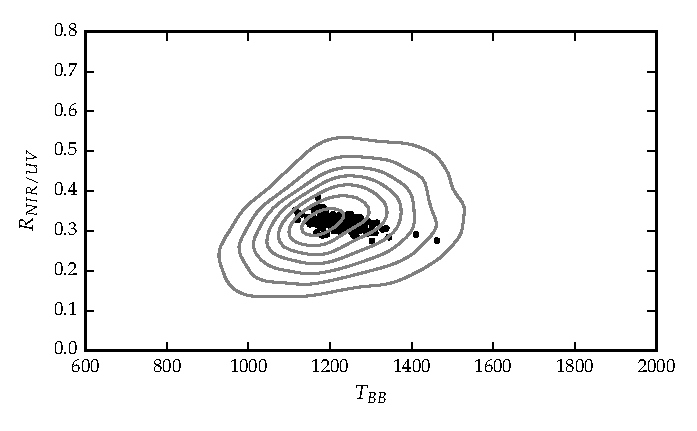
\includegraphics[width=\textwidth]{figures/chapter06/ratio_tbb_contours.pdf}
  \caption{Ratio of NIR to UV luminosity ($R_{NIR/UV}$) against temperature ($T_{BB}$). The grey contours show equally-spaced lines of constant probability density generated using a Gaussian kernal-density estimator on our data sample. The black points are for our mock data.}
  \label{fig:}
\end{figure}

We now look for correlations between the properties of the black-bodies we have fitted to the hot dust emission and other properties of the quasar such as redshift, black-hole mass, and normalised accretion rate (Eddington ratio). 

Firstly, we test whether the properties of the black-body evolve with redshift. 
In the Figure in the proceding section we plotted the temperature of the black-body component of our model as a function of redshift. 
This reveals evidence for a weak anti-correlation between the black-body temperature and the redshift ($\rho =$ -$0.09$, $p = 2e$-$10$). 
It could be that this apparent trend is an artifact of the fitting procedure. 
Although we constrained the redshift range of the sample specifically to mitigate for such an effect, the region of the rest-frame spectrum being fit is changing systematically as a function of redshift. 
To test this we fit a mock data set of SEDs with fixed black-body properties at a range of redshifts. 
The best-fit black-body temperatures are shown with the dashed black line in the Figure. 
There is no evidence for any change as a function of redshift. 
Furthermore, we showed in an above Figure that there is no evidence for any systematic change in the quality of the fit with redshift. 
Of course, redshift and luminosity will always be correlated for a flux-limited sample such as this. 
Therefore we will now look for correlations of between the black-body temperature and luminosity, as well as the black-hole mass and Eddington ratio.  

\begin{figure}
  \centering
  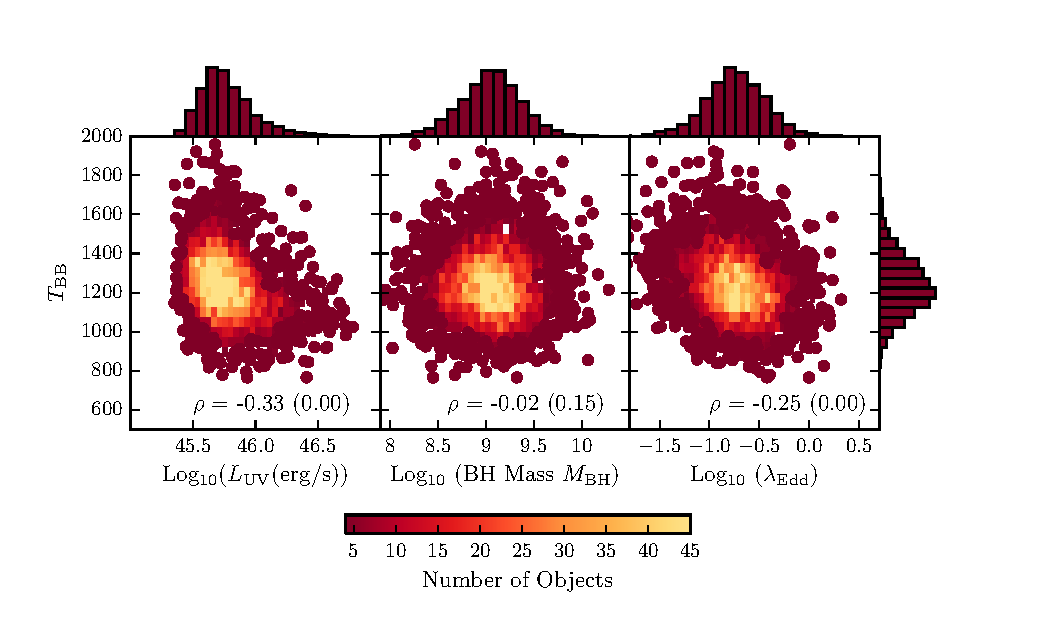
\includegraphics[width=\textwidth]{figures/chapter06/tbb_lowz_correlations.pdf}
  \caption{Best-fit black-body temperature against UV luminosity (left), black-hole mass (center) and Eddington ratio (right). We also quote the Spearman rank correlation coefficients and p-value for a hypothesis test whose null hypothesis is that two sets of data are uncorrelated.}
  \label{fig:}
\end{figure}

There is a clear anti-correlation between the UV luminosity and the best-fit black-body temperature. We calculated a Spearman rank-order correlation coefficient -0.33. The fact that the blackbody temperature is anti-correlated with the luminosity could explain the weak anti-correlation between black-body temperature and redshift we saw in the Figure above. 

The black-hole masses are virial estimates calculated by Shen et al. 2011 using the MgII emission line in the SDSS spectra. There is no evidence for a correlation between the best-fit black-body temperature and the black-hole mass ($\rho=$-$0.02$, $p=0.15$).  

The Eddington ratios (bolometric luminosity normalised by Eddington luminosity) are also calculated by Shen et al. 2011 using bolometric corrections in Richards et al. (2006a) using 3000A monochromatic luminosities. 
There is a clear anti-correlation between the best-fit black-body temperature and the Eddington ratio ($\rho=$-0.25, $p=2.4e$-64). 
Given what we know about the trends of black-body temperature with luminosity and black-hole mass, this is to be expected. 
Eddington ratio is proportional to luminosity, which is anti-correlated with black-body temperature, and inversely proportional to the black-hole mass, which has no correlation with black-body temperature. 
Therefore it is to be expected that black-body temperature is anti-correlated with the Eddington ratio. 

Next, we look for correlations of some of the fundamental properties of quasars with the ratio of NIR to UV luminosity. 
In the previous section we showed a possible anti-correlation between the black-body temperature and the UV luminosity. 
As we discussed in an earlier section, the luminosity of hot dust is correlated with the temperature, such that lower-temperature hot dust has a greater luminosity. 
We emphasise this point in the Figure below, where we plot the ratio of NIR to UV luminosity against the black-body temperature, colour-coding the points by the UV luminosity. 
The UV luminosity changes most strongly as a function of temperature, but there is also a much weaker correlation with the NIR to UV luminosity ratio. 
We calculated a partial Spearman rank correlation coefficent of 0.10 after the mutual dependence of the NIR to UV luminosity ratio and the UV luminosity on temperature had been factored out. 
Another way of showing this is to take slices of constant temperature; this is shown in the Figure below. 
There is a very weak correlation, although it is not clear whether it is statistically significant. 
Note that by restricting the redshift range we are limiting the dynamic range in luminosity, which may be why we don't see the stronger trend observed by Roseboom et al. 

A particularly important issue is to deduce whether $L_{UV}$ or $T_{BB}$ is the primary parameter with which $R_{NIR/UV}$ correlates. 
We approach this problem in two ways; the first is to carry out correlations in separate $L_{UV}$ or $T_{BB}$ intervals, removing any possible spurious correlations with the remaining independent variable. 
The second approach is to use partial Spearman rank correlation (e.g. Macklin 1982) to derive the correlation coefficient holding one independent variable constant: 

$ \rho_{AX,Y} = \frac{ \rho_{AX} - \rho_{XY}\rho_{AY} } { \sqrt{ ( 1 - \rho^2_{XY} )(1 - \rho^2_{AY})} } $
 
where X and Y are two independent variables (e.g. $L_{UV}$ and $T_{BB}$ ) and A is the dependent variable (e.g. $R_{NIR/UV}$). 
$\rho_{AX}$ , $\rho_{AY}$ and $\rho_{XY}$ are the Spearman correlation coefficients for the separate correlations between two variables. 
The significance of $\rho_{AX,Y}$ is given by

$ D_{AX,Y} = \frac{\sqrt{N-4}}{2}{\rm ln} \left( \frac{ 1 + \rho_{AX,Y}}{ 1 - \rho_{AX,Y}} \right) $

which is distributed normally about zero with unit variance (Macklin 1982), where N is the size of the sample. 
In using this partial rank correlation approach we are testing the null hypotheses that i) the $R_{NIR/UV}$-$L_{UV}$ correlation arises entirely from the $R_{NIR/UV}$-$T_{BB}$ and $T_{BB}$-$L_{UV}$ correlations, and ii) the $R_{NIR/UV}$-$T_{BB}$ correlation arises entirely from the $R_{NIR/UV}$-$L_{UV}$ and $R_{NIR/UV}$-$T_{BB}$ correlations. 
If the coefficients for the $R_{NIR/UV}$-$T_{BB}$ correlation are larger than those for the $R_{NIR/UV}$-$L_{UV}$ correlation, this would imply that $R_{NIR/UV}$ is primarily correlated with $T_{BB}$.

Looking at Figure 17 in summary-150309, there is such a small dymanic range in the UV luminosity - only 0.5 dex. 
Given the size of the errors on the luminosity I would be surprised if we saw any correlation. 

Assuming that the NIR emission really is coming from a cloud emitting at a single temperature then we can integrate the whole of the black-body curve to give us a NIR luminosity. 
However, this is probably not true, in which case it might be more appropriate to use the black-body soley as a good parameterisation of the shape of the SED in the 1-3$\mu$m region, and to calculate the NIR luminosity in a more limited wavelength range. 
This is shown in the Figure below. 
There are no significant correlations with either the UV luminosity, black-hole mass or Eddington ratio. 

I have a quite small dynamic range in luminosity, so maybe I can combine this with high-$z$ to see correlation. 
As first step see if there is a difference in the median $R_{NIR/UV}$ for low/high luminosity samples. 


\begin{figure}
  \centering
  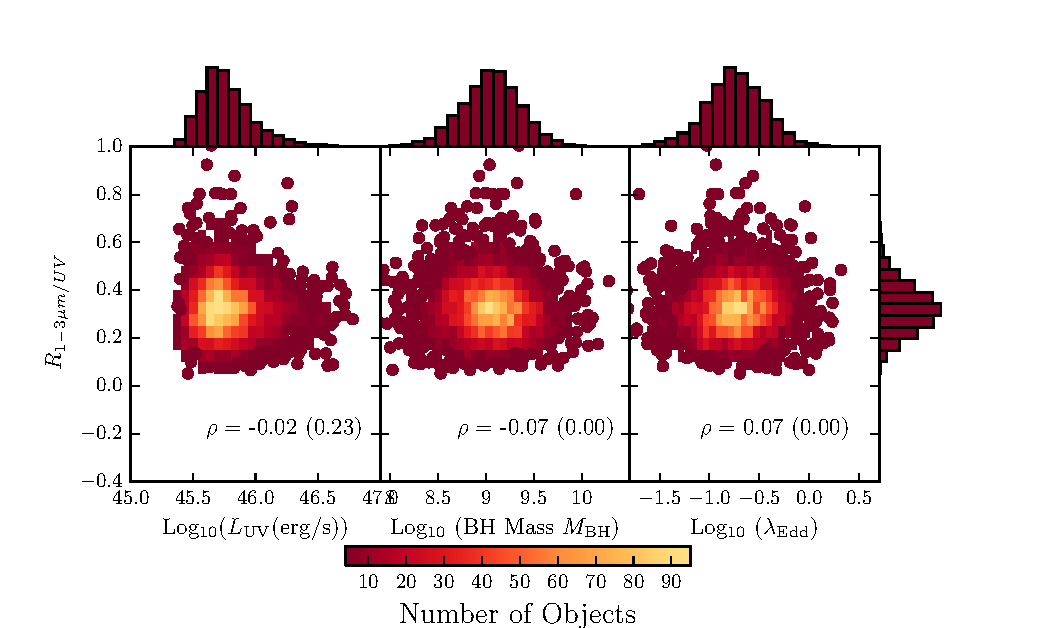
\includegraphics[width=\textwidth]{figures/chapter06/ratio_lowz_correlations.pdf}
  \caption{Black-body luminosity calculated between 1-3 $\mu$m.}
  \label{fig:}
\end{figure}

\begin{itemize}
\item Demonstration of range of T\_BB and normalisation - OK. Again, various caveats re: wavelength-range, etc could be covered earlier.
\item Make clear in write-up redshift-range contributing to each plot.
\item So - do we believe there is a real trend in the lh panel?
\item Then, take Roseboom's trend - would it be visible in the colour-coded figure?
\item* Should discuss the use of different near-IR luminosities, including integral under BB-curve. Probably makes more sense to present the figure with luminosity from 1-3 microns and then introduce the "Suppose we really do have a true BB-component..." and present previous plot.
\end{itemize}

\subsection{High-$z$ correlations}

We will now perform a similar analysis on our high-$z$ sample. We showed in a previous section how in the redshift range $2 < z < 2.7$ the black-body parameters do not change as a function of redshift. Below we plot the black-body parameters against UV luminosity, black-hole mass and Eddington ratio. 

At low-$z$  we get a much larger range in black-body temperatures from our fits. We discussed how the W3 S/N > 5 cut might be be biasing the high-z sample if the subset being removed had properties distinct from the remainder of the sample. The W3 S/N > 5 cut removes about 25\% of the sample. 

\begin{figure}
  \centering
  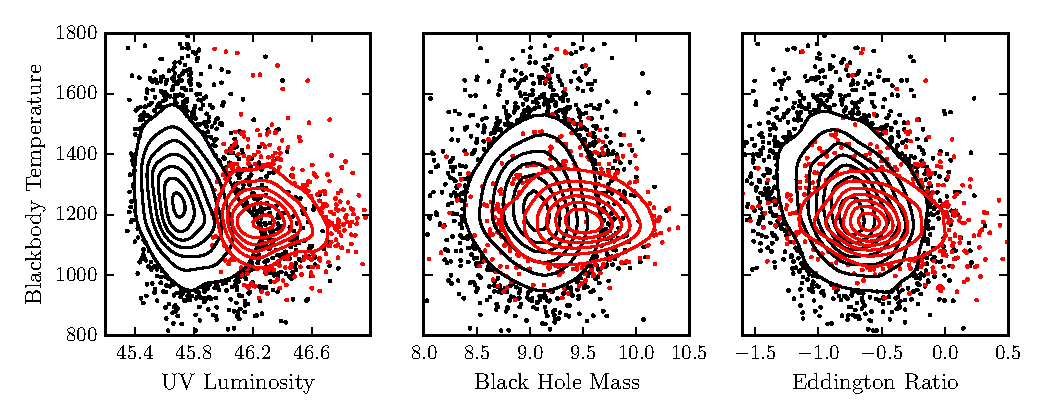
\includegraphics[width=\textwidth]{figures/chapter06/bbt_correlations_contour.pdf}
  \caption{Black-body temperature and UV luminosity, black-hole mass and Eddington ratio. Black is low-$z$ sample and red is high-$z$ sample. In region of high-density we represent the density with contours, which are smoothed using Gaussian kernel density estimation.}
  \label{fig:}
\end{figure}

\begin{figure}
  \centering
  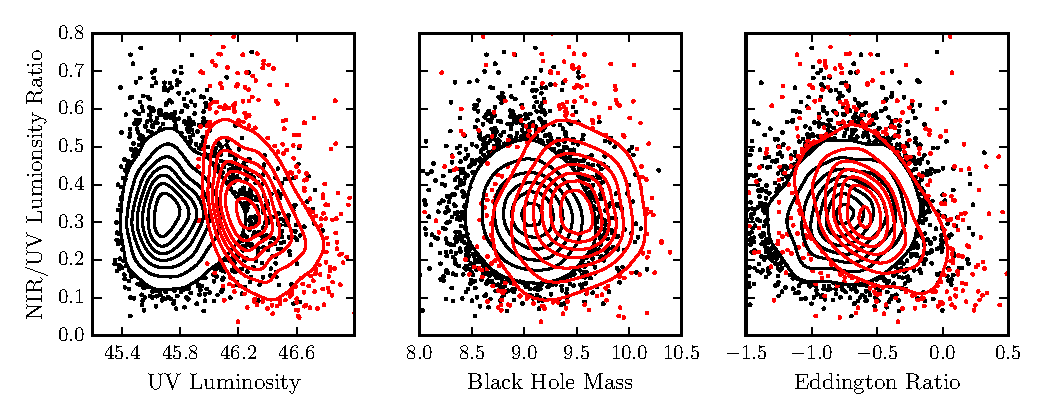
\includegraphics[width=\textwidth]{figures/chapter06/ratio_correlations_contour.pdf}
  \caption{Ratio of NIR to UV luminosity and UV luminosity, black-hole mass and Eddington ratio. NIR calculated 1-3$\mu$m. We expect the black hole masses to be overestimated in quasars with more hot dust. }
  \label{fig:}
\end{figure}

We observe a postive correlation between the black-hole mass and the NIR to UV luminosity ratio which is quite different from what we observed in our low-$z$ sample. 
We believe that this is just a manifestation of the fact that at high redshift the black-hole masses are derived from CIV. 
We will show below how the FWHM of CIV has a positive correlation with the hot dust abundance, and large CIV FWHM leads to larger black hole mass estimates. 
This explains the apparent correlation between the IR/UV ratio and the black hole mass. 
Eddington ratio measures the luminosity relative to the Eddington luminosity. 
Higher blackhole mass estimates will lead to lower Eddington ratios, which is why the Eddington ratio appears to decrease with increasing IR/UV ratio. 
For the sources in our low-$z$ sample the black-hole mass is measured using the broad MgII emission line. 
As we will show below, the properties of the MgII emission line have no dependence on the hot dust properties. 

\subsection{Power-law fot to NIR emission}

In this next section I model the NIR emission using a single power-law. 
This has been done by other authors (e.g. Wang et al., Zhang et al.). 
I want to compare the relative effectiveness of the black-body and power-law in parameterising the NIR emission. 

The power-law is normalised at 9000A, where its flux is set equal to the flux of the UV/optical model. 
The NIR power-law slope is fit between 1 and 2.4$\mu$m (although the exact wavelength region being fit depends on the redshift of the quasar). 
At 9000A we are dominated by direct emission from the accretion disc. 
Therefore we can interpret $\beta_{NIR}$ as being the ratio of hot dust to accretion disc emission. 

\begin{figure}
  \centering
  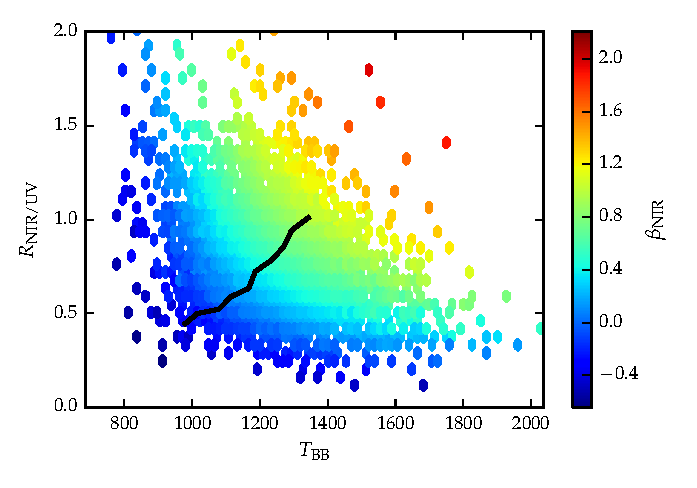
\includegraphics[width=\textwidth]{figures/chapter06/ratio_tbb_beta.pdf}
  \caption{IR to UV lumiosity ratio against temperature of blackbody, colored by the power-law slope from fit to low-$z$ sample. The black line gives an indication of how $\beta$ changes as a function of the other parameters. Note NIR luminosity calculated by integrating black-body over all wavelengths.}
  \label{fig:}
\end{figure}

If we plot the normalised residuals from power-law fit against $\lambda_{eff}/(1+z)$, the residuals clearly vary systematically with the rest-frame wavelength, or equivalently redshift. 
From this we can conclude that the black-body is a better fit to the shape of the NIR emission than the power-law. The fact that the quality of the fit changes as a function of redshift for the power-law could lead to errenous results when looking for correlations of the power-law index with other properties of the quasar. 

I need to decide here whether to show results from my power-law fit with a truncated UV/Opt power-law emission (and fixed NIR power-law normalisation) or from my fit where NIR power-law is an additional component in model with free normalisation.  

We need to talk about beta as used by Wang and Gallagher et al. but Gallagher et al. establish the curvature in the SED is a problem [which we could illustrate via one of your residual plots]. 
Again. something we should almost certainly establish early on, with a view to justify what we will/won't use to model the SEDs and what we do/don't believe from the literature that employs beta-fits.
Should definitely review the source (and limitations) of the various fundamental quasar/black-hole parameters early-on - including M\_BH and the MgII-CIV systematic.

\subsection{Correlation with outflow properties}

Previous studies have suggested a link between dust and outflows. 
For example, BAL quasars are typically redder than non-BAL quasars, which many authors attribute to enhanced dust extinction. 
Furthermore, quasars with large CIV blueshifts are on average bluer than quasars with smaller CIV blueshifts (Reichard et al. 2003). 
Dust absorption could be an important acceleration mechanism for dusty outflows. 
It could be that outflows originally contain dust or dust is produced in the outflows. 
Alternatively, outflows might interact with the dusty torus and strip of dusty gas. 
Or there could be no direct relation between dust and outflows, but both could depend simultaneously on a third property, such as the Eddington ratio. 

At redshifts $1 < z < 1.5$, the SDSS spectra cover the rest-frame region ~1000-4000A. 
The most prominent broad emission line in this region is MgII${\lambda}{\lambda}$2796,2803. 

\begin{figure}
  \centering
  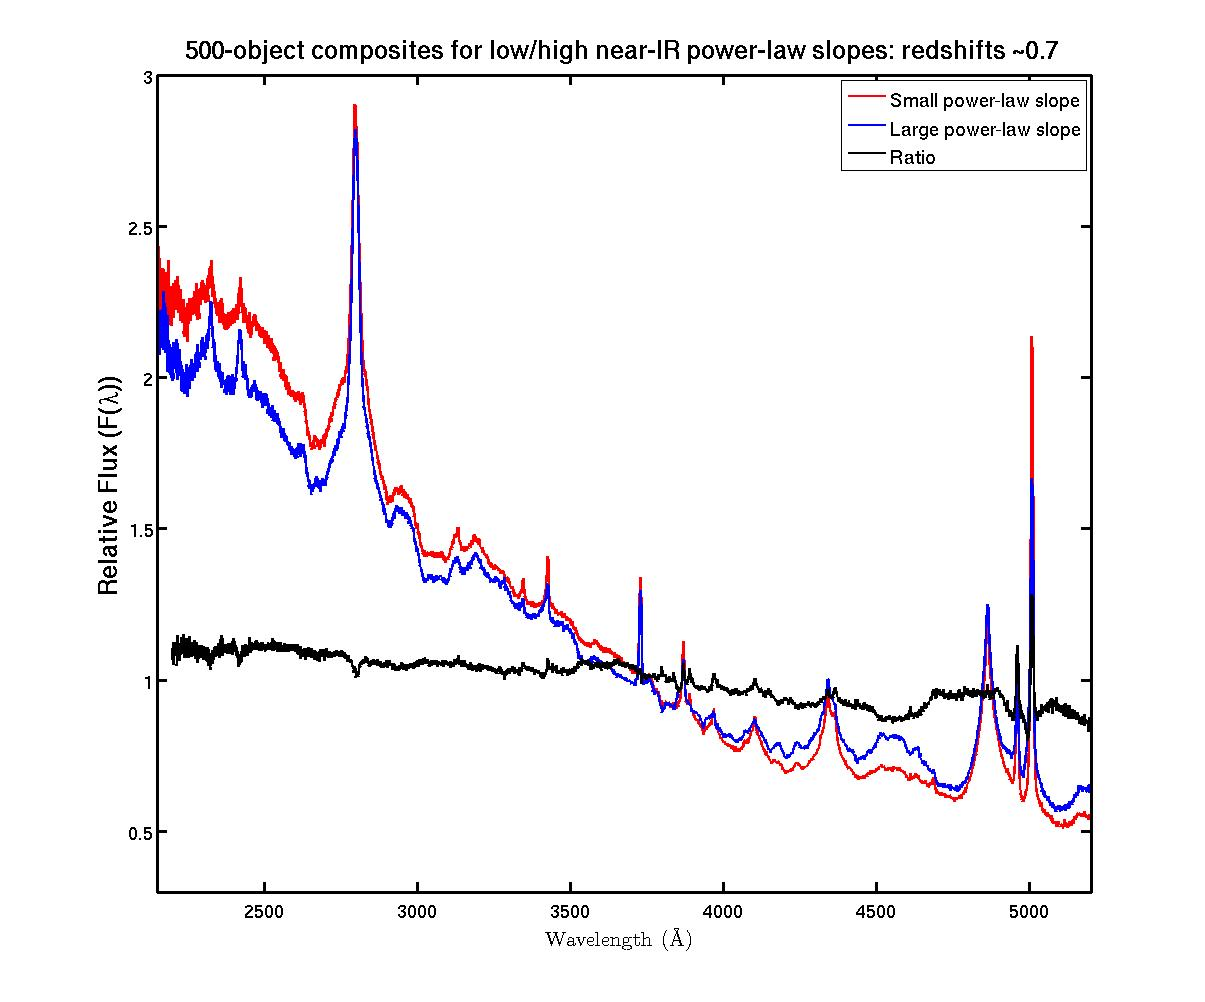
\includegraphics[width=\textwidth]{figures/chapter06/z07_pls_comps.jpg}
  \caption{Composite SDSS spectra for objects at $z\sim0.7$. We have divided sample into objects with objects best-fit by small (red line) and large (red line) values of $\beta$. Change this to select by $R_{NIR/UV}$ / $T_{BB}$. Label prominent emission lines. This is below the redshift limit of my low-$z$ sample, and so I need to justify its inclusion. We don't see any significant changes in the [OIII] FWHM, which we might expect following Shen \& Ho 2014. }
  \label{fig:}
\end{figure}

The $z < 0.8$ SDSS spectrum composite comparison for the small and large $\beta_{NIR}$ sub-samples is a very direct illustration of the Boroson \& Green 1992 Eigenvector 1 describing the spectral variation in the optical spectra of quasars; as FeII EW increases the [OIII] EW decreases. 
Hot dust emission increases with FeII EW (Shen \& Ho 2014). 
We also note that the amount of hot dust correlates with the SiIII/CIII] emission ratios. 
The Si iii]/Ciii] ratio is generally considered to be a good indicator of density and is one of the primary EV1 correlates. 
The relative flux ratio of Si III] to CIII] increases when CIV is more blue-shifted (Richards et al. 2011). 
Unlike CIV for the high-$z$ sample, MgII emission line has exactly the same profile/shape for the two samples (change in MgII width for z$\sim$ 0.7 sample more to do with change in FeII at wavelengths just shortward of the line). 
Finally, we note that objects with more hot dust are slightly redder.

For our high-$z$ sample CIV$\lambda$1550 is redshifted into the SDSS spectrum. 
In the Figure below we show how the ratio of NIR to UV luminosity depends on the blueshift and rest-frame equivalent width of the CIV line. 
The CIV emission line blueshift is obtained from the wavelength of the centroid of the emission line relative to the predicted location for emission at the systemic velocity of each quasar. 
Systemic redshifts are obtained from Hewett and Wild (2010).

\begin{figure}
\centering
  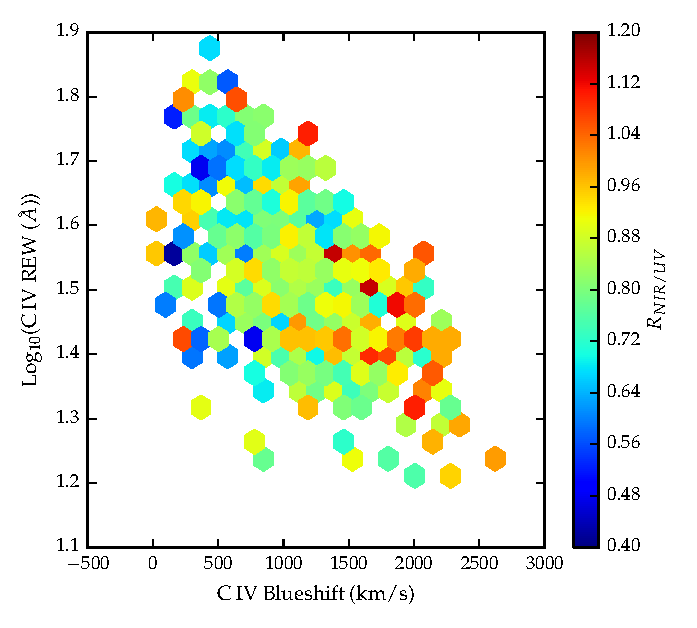
\includegraphics[width=\columnwidth]{figures/chapter06/hot_dust_ratio.pdf}
\caption{CIV rest-frame equivalent width versus blueshift for our high-$z$ sample. Color indicates the mean best-fit value for the NIR to UV luminosity ratio for the objects located in the hexagonal bin. Only bins containing a minimum of two objects are plotted. This is different sample to the one used in the beta version (see below). Need to investigate differences and hopefully get a good figure without using beta.}
  \label{fig:}
\end{figure}

We see that the NIR to UV luminosity ratio is strongly correlated with the blue-shift of the CIV emission line. 
A similar trend was noted by Wang et al. 2013. 

We see strong systematic change in the emission-line properties of the CIV emission line as a function of the near-IR power-law slope. 
Interestingly, we note strong similarities to the object subsets selected according to their CIV-emission properties in Richards et al. 2011 (see Figures 11 \& 12).  

In the composite spectra above we see a clear non-virial component to CIV line, which depends systematically on the hot dust abundance. 
We believe this effect to be responsible for the correlation between hot dust abundance and black-hole mass we observed above. 

Here we focus in on the high ionisation broad CIV emission line, where differences in the line profile are the most noticeable. 
We observe that objects with larger amounts of hot dust emission have very different CIV line profiles from objects with smaller amounts of hot dust emission. 
For objects with larger amounts of hot dust emission the line is skewed, and peaks at slightly shorter wavelengths. 
This line profile is indicative of stronger accretion disc winds. 
The fact that there is a correlation between the amount of hot dust we see and the strength of the accretion disc wind could indicate that there is a hot dust component in the wind. 
The difference was apparently larger when initially using beta. 
Liam has on his list to understand why the beta-related trend is apparently stronger than with the blackbody parameters.

\subsection{BALs and radio-loud/radio-quiet}

In the spectra of about 20\% of all quasars we observe broad (> 2000km/s) blue-shifted absorption troughs which are associated with quasar-driven out-flowing gas. BAL quasars in general have redder UV continua than non-BAL quasars, which is interpreted as the result of dust extinction. BAL quasars, on average, also have higher Eddington ratios and luminosities than non-BAL quasars.

We defined a sample of BAL quasars using the same method we used to define our sample of non-BAL quasars. Need to justify our use of model which has been optimised to fit colours of non-BAL quasars, when we know that BALs are typically redder. At $1 < z < 1.5$ there are very few BAL quasars in our sample. In the $2 < z < 2.7$ redshift region we have 394 HiBAL quasars (the wavelength coverage of the SDSS spectra are not sensitive to LoBALs at these redshifts). What catalogue did we use to define quasar sample? Since BAL quasars are expected to suffer more from extinction due to dust, we have allowed E(B-V) to vary for the BAL quasar sample. 

We find that the black-body temperature distributions are consistent (median $T_{BB}$ for both samples = 1180K), but the ratio of NIR to UV emission is higher in BALs ($R_{NIR/UV}$ = 0.92 and 0.83 for BAL and non-BAL quasar sample respectively). This is qualatatively consistent with the results of Zhang et al. 2014. 

It is well known that the blueshift of the CIV emission line in radio-quiet AGNs is, on average, stronger than in radio-loud AGNs (Marziani et al. 1996; Sulentic et al. 2000a; Richards et al. 2002, 2011). Statistically at least, the "radio-loud" objects are thought to have high black-hole masses and there is some form of radio-mode feedback (jet related) which is very different from the much more common (almost certainly wider opening-angle) outflow objects with large CIV-blueshifts.

So we find BALs have more hot dust, radio-loud have less. 
This is perfectly consistent with what we know about the positions of radio-loud objects and BALs in the CIV parameter space distribution (Richards et al. 2011). 

\section{Discussion}

\subsection{Anti-correlation between black-body temperature and quasar luminosity} 

At low-$z$, $R_{NIR/UV}$ independent of quasar luminosity. 
At high-$z$, $R_{NIR/UV}$ anti-correlated with quasar luminosity. 

Roseboom et al. 2013 studied a similar sample of luminous type 1 quasars. 
They, like us, modelled the NIR emission using a black-body and modelled the emission at longer wavelengths using a clumpy torus model. 
They find that while $L_{1-5\mu m}$/$L_{IR}$ appears relatively insensitive to $L_{bol}$ and $L_{IR}$, a strong correlation appears between $L_{1-5\mu m}$/$L_{IR}$ and $L_{IR}/L_{bol}$ (i.e. the dust covering factor). 
As the covering factor decreases, the maximum inclination at which a type 1 quasar would be seen increases. 
An increase in the inclination will mean direct sight lines to more of the inner wall of obscuring material closest to the accretion disc.

Mor \& Trakhtenbrot 2010 also looked at the hot dust properties of a sample of $0.75 < z < 2$ quasars, with photometry from SDSS and WISE. 
They modelled the NIR emission with hot clouds of pure graphite dust. 
They reported an anti-correlation between the covering factor of hot dust clouds and the quasar bolometric luminosity. 
Like us, they neglect cooler dust components which will dominate the SED at longer wavelengths. 
As we have discovered (see Figure residual plot), the missing flux decreases with redshift because we observe shorter rest-frame wavelengths when the observed spectrum is redshifted to a greater degree. 
This will induce an anti-correlation between the luminosity of the hot dust component and the luminosity of the quasar (which is correlated with redshift). 
At z=0.75, the W3 band-pass (the longest in their fits) is sensitive to flux from 6.9$\mu$m; at this wavelength we expect the contribution from cooler dust to dominate over the hot dust. 
It is possible that this effect could explain the tension with our own result that $R_{NIR/UV}$ does not depend on the quasar luminosity in our low-$z$ sample. 

Shen \& Ho 2014 quantify the relative torus emission using the $r-W1$ colour for a sample of $0.4 < z < 0.8$ SDSS quasars. 
At these redshifts W1 is observing between 1.9 and 2.4 microns in the rest-frame of the quasar, which suggets that they are sensitive to the same component of hot dust which we are investigating. 
They observe a mild trend of decreasing relative torus emission as the quasar luminosity increases. 
We note that their use of the r-W1 at much higher redshifts may be problematic, as the W1 flux will be increasingly dominated by direct emission from the accretion disc. 

Gallagher et al. 2007 undertook a similar investigation for a much smaller sample of 234 radio-quiet quasars.

\subsection{Eddington ratio}

At low-$z$, I find that the black-body tempearture is anti-correlated with the Eddington ratio, but at high-$z$ I find no correlation. 
At low-$z$ I find no correlation between $R_{NIR/UV}$ and the Eddington ratio, but at high-$z$ I observe an anti-correlation. 

Wang et al., Zhang et al., and Mor \& Trakhtenbrot find no significant dependence of the amount of hot dust on the Eddington ratio. 

Shen \& Ho find that torus emission is enhanced in quasars with larger $R_{FeII}$. 
They show how EW(OIII) and other high-ionisation lines (and to a lesser extent low-ionisation lines like MgII) anti correlate with $R_{FeII}$. 
The enhancement of torus emission relative to accretion disc emission at the high-RFeII end of EV1 may be caused by more efficient disc winds that facilitate the formation of a dusty torus. 
From our $z\sim0.8$ composite SDSS spectra, we observed that objects with large NIR to UV luminosity ratios on average have stronger FeII emission. 
[OIII] has anti-correlation with FeII, and so does MgII to a lesser extent. 
So I would expect the hot dust emission to anti-correlate with the EW of MgII, at fixed luminosity. 
However, I find that the MgII EW is independent of the hot dust luminosity. 

\subsection{Schemes that depend on viewing angle}

Disc emission is theoretically predicted to scale with the cosine of the disc inclination angle. 
If hot dust emission is (approximately) isotropic, the amount of hot dust emission relative to the accretion disc emission is expected to increase with increasing IA. 
However, the dust torus may block the hot dust emission at large IA (Roseboom et al. 2013). 
It complicates the situation and makes the dependence of $R_{NIR/UV}$ on IA uncertain. 
Runnoe et al. 2013 investiaged the inclination dependence of quasar SEDs. 
Their Figure 6 llustates that an edge on quasar spectrum tends to show a slightly enhanced NIR bump.

Shen \& Ho observed that, at fixed $R_{FeII}$, torus emission is enhanced when $FWHM_{H\beta}$ increases. 
H$\beta$’s width relates to the orbital velocity of gas along our line of sight. 
They conclude that H$\beta$'s width reveals the orientation of the quasar's disc to our line of sight, with a wider line corresponding to a more edge-on disk. 
The width of other broad emission lines (e.g. MgII) should show the same dependance.   
   
\subsection{Black-body better fit to NIR emission than power-law}

\subsection{EV1 Correlations}

According to the Eigenvector 1 trend, first identified by Boroson and Green in 1992, quasars with strong optical Fe II emission have weak emission from [OIII]. 
The systematic correlations suggest that a single physical parameter drives Eigenvector 1, which is believed to be the Eddington ratio. 
BAL quasars have more hot dust on average
Radio quasars have less hot dust on average

\subsection{Gordon's model}

Assume that the dusty torus is just the extension of the wind beyond the dust sublimation radius.  
Start with a Konigl \& Kartje MHD wind that is roughly polar.  
The hot dust then forms a sort of vertical "wall" around the accretion disk.  
Now crank up the UV photons and turn on radiation line driving, giving you a Murray \& Chiang wind. 
That flattens the geometry of the wind and exposes more surface area that is viewable on a relatively face-on line of sight.  
So you are able to see more of the dust that is closest in.

\subsection{Dust-Free Outflow Scenario}

Correlations shown in Wang et al. and Zhang et al. could be induced by a third factor that simultaneously governs or relates to outflows and dust emission. 
Assume that hot dust emission is not directly related to outflows and is predominantly emitted by the innermost part of a hydrostatic and optically thick torus, as suggested by lots of previous studies.

1. Outflow strength is significantly dependent on the Eddington ratio, broadband SED (e.g. ionisation SED, UV continuum slope, $\beta_{UV}$) and luminosity. 
If these factors also have an impact on the hot dust emission, one might find a piece of evidence to support the dust-free outflow scenario. 
As shown in Zhang et al., Wang et al., Mor \& Trakhtenbrot, $\beta$ is almost independent of the Eddington ratio. And no correlation with luminosity. 

2. Metallicity. Quasars harboring strong outflows tend to have high gas metallicity. 
Wang et al. (2012) found that CIV blueshift increases with gas metallicity. 
Since dust forms more easily in higher metallicity gas, one may expect that metallicity is an appropriate factor which simultaneously influences outflow and hot dust emission. 
However, for a typical torus, the relative amount of dust emission is determined by the dust covering factor but not by the dust amount. 

\subsection{Dusty outflows}

BALs are on average redder than non-BAL quasars and quasars with large CIV blueshift are on average bluer than those with small blueshift. 
Since BAL and BEL outflows very likely represent the same physical component, this seeming contradiction can be reconciled by a special geometrical configuration in which dust is associated with outflows. 
In this case, dust reddening is preferably observed in the outflow direction (Wang et al.) 

Either outflows originally contain dust or dust is manufactured in outflows (Elvis et al. 2002). 

1. Dust is intrinsic to outflows. 
The idea is supported by the similar locations of BAL outflows and hot dust. 
Reverberation mapping results suggested that hot dust is located at the outer boundary of BEL regions (Suganuma et al. 2006). 
The outflow launching region is also suggested to be co-spatial with or outside of the BEL regions. 
Outflows may emerge from the outer region of the accretion disc or even the innermost region of the torus, in which the gas clouds are dusty and relatively cold. 
The dusty clouds are uplifted above the disk and are exposed to the central engine. 
The low density part is highly ionized and responsible for the blueshifted absorption and emission lines. 
Dust survives in the dense region and radiates in the NIR band. 
The dust carried by outflows is heated by the central engine to emit at the sublimation temperature, meanwhile dust absorption contributes to the outflow acceleration. 

2. Outflows interact with torus clouds. 
The process makes more dust in the clouds exposed to the central source. 
As a consequence, the IR emission increases, and the outflows become dusty. 
Since a stronger outflow can ablate dense clouds more effectively, the dependence of NIR emission on outflow strength is yielded. 
In this scenario, outflows confine the geometry and subtending angle of the dusty torus. 
One problem is that the interaction timescale is much shorter than the quasar lifetime. 
The correlation might disappear after outflows blow away all of the clouds in the outflow direction. 

\subsection{Gallagher et al.}

From plot looks like higher luminosity objects have higher temperatures, which is opposite of my trend. 
See if I can find these objects in SDSS and do my own fits. 
Found them, but I think I needed to modify my code for the Spitzer photometry. 

IR/UV luminosity decreases with increasing UV luminosity, but lower-luminosity more likely to have more extinction and more extinction means a higher IR/UV ratio. 

Dynamic range in lumionosity is much bigger than I have in my sample, so I might not expect to see such a strong trend. 

I really like the "torus as the dusty part of the wind" idea that a number of people have been pushing. 
Starting with Konigl \& Kartje 1994, but extending to more recent work by Everett and Elitzur.

For example:

\begin{itemize}
\item http://adsabs.harvard.edu/abs/2009AIPC.1201...56E
\item http://adsabs.harvard.edu/abs/2012ASPC..460..199G
\item http://adsabs.harvard.edu/abs/2005ApJ...631..689E
\item http://adsabs.harvard.edu/abs/2012ApJ...749...32K
\item http://adsabs.harvard.edu/abs/2006ApJ...648L.101E
\end{itemize}

For "where is the dust", some good references are

\begin{itemize}
\item http://adsabs.harvard.edu/abs/2008ApJ...675..960P
\item http://adsabs.harvard.edu/abs/2007ApJ...671..124D
\end{itemize}

It would be interesting to see how Coleman's "corrected" spectral indices match up with your T\_BB values.
You say that there is no correlation of T\_BB with E(B-V), but if there is a correlation with R\_NIR/UV (I beg you to use alpha\_niruv instead -- I'm on a mission to do away with "log R" in the radio too, see my tirade in Kratzer \& Richards 2015), then there must be a correlation with alpha\_opt.  
And if I am right that bluer objects are more likely to be dust reddened, then I might that expect to show up in T\_BB vs. E(B-V) (at least in a subsample).  
So I'm surprised that Fig. 36 doesn't show more of a difference.

For radio/orientation, Kratzer \& Richards 2015 says pretty much everything that I think/know.  
A student is looking into extending that analysis to BALs.  
And I'm very keen to take advantage of the new S-band VLA data on Stripe 82 to compute spectral indices to use as orientation indicators.  
Just need to get the data from the PI....

Oh, before I forget: I haven't read any of the papers by Makoto Kishimoto, but after Willsfest in Austin where he presented some of his work, I feel like I'm really missing out by not having done so. In addition to a number of recent papers, his talk from that meeting is at http://www.as.utexas.edu/quasars/talk\_kishimoto\_m.pdf. I was particularly interested in Slide 12.

In Figure \ref{fig:w1w2colors} we plot the $W1 - W2$ colors of the DR7Q-matched sample as a function of redshift from $z=0.2$ to $z=1.8$. In this redshift range the $W1$ and $W2$ band-passes are probing the 12,000 - 28,000 \AA~ and 16,000 - 38,000 \AA~ region of the rest frame SED respectively, and the $W1-W2$ color is therefore predominantly tracing emission from hot dust at temperatures $\sim 1200$ K. At any given redshift or, equivalently, region of the rest-frame SED, we see a $\sim 0.5$ mag dispersion in the $W1-W2$ colors. On the same axes in Figure \ref{fig:w1w2colors} we have plotted the $W1 - W2$ colors derived from our SED model with blackbody temperatures ranging from 1000 - 1600 K and blackbody normalisation factors (i.e. the flux from the blackbody component relative to the power-law continuum at a reference wavelength) from 0 - 0.5, with the other parameters as reported in Table \ref{tab:params}. A blackbody with a single temperature and normalisation is clearly not a very good representation of the hot dust properties of the whole sample. We aim to study the diversity hot dust properties of the quasars in our sample to learn about the nature of the hot dust, and to link the hot dust properties to other physical quantities such as the luminosity and redshift of the quasar. 

We decided to explore the diversity of hot dust properties by fitting our standard model, with the blackbody temperature and normalisation as free paramters, to the individual quasar SEDs. 




The first step was to define a sample of quasars from the DR7Q-matched catalogue which were well fit by our standard un-reddened SED model. To achieve this we discarded from our sample quasars with $i - K$ colors redder than our standard model with dust reddening E(B-V) = 0.1. This region of the $i-K$ colour space includes both quasars with significant amounts of dust redenning and quasars with extreme emission line equivalent widths. We exclude quasars with observed magnitudes fainter than 19.1 in the $i$ band-pass, as well as quasars with upper-limit or S/N $<$ 5 magnitudes in the $K$, $W1$ and $W2$ band-passes (without these we will be unable to properly constrain the blackbody slope). We exclude quasars flagged as broad-absorption line quasars \citep[BALQSOs;][]{weymann91} from the sample, since these objects may be in a special evolutionary stage and have different hot dust properties. Finally, from all of the objects which passed the above criteria, we discarded the 10\% of quasars which were least well fit by our standard model.   

It is important to consider the redshift range over which we can reasonably expect to be able to constrain the shape of the blackbody component. The amount by which the observed spectrum is redshifted determines the position of the hot dust feature in the spectrum relative to the wavelength coverage of our set of band-passes. For a redshift $z \sim 1.5$ quasar, only the $W2$ band-pass, at $\sim 2 \mu$m in the rest frame of the quasar, is probing the wavelength region dominated by the blackbody emission (the peak in a $T \sim 1200$K blackbody is at $\sim 2.4 \mu$m). At $z \gtrsim 1.5$, we found that we could no longer constrain the shape of the blackbody component in our SED model using the $ugrizYJHKW1W2$ band-passes. Although we could include magnitude constraints from the longer-wavelength WISE $W3$ band-pass ($\lambda_{\rm eff} \simeq 12 \mu$m), at $z \sim 1.5$ this is observing $\sim 5 \mu$m in the quasar's rest frame. In this region there will be extra contributions to the flux, possibly from cooler dust, which are not accounted for in our model. This was clearly demonstrated by the increase in the $m_{\rm model} - m_{\rm data}$ residuals beyond $\sim 3\mu$m in the rest frame. At lower redshifts, the $W3$ band-pass is probing even longer-wavelengths, where the component we are missing from our model will be greater. To compensate our SED model will move the blackbody component to lower temperatures, which shifts the peak to longer wavelengths. The result will be a downward trend in the blackbody temperature with decreasing redshift. Given that one question we are interested in addressing is variations in the hot dust properties with redshift, we have to be very wary of systematic effects such as these. With these considerations in mind, we restricted ourselves to determining the hot dust properties of our quasar sample in the redshift range $0.5 < z < 1.5$. 

In Figure \ref{fig:residuals} we saw how the model appeared to be underestimating the observed flux in the region around $1\,\mu$m in the quasar rest frame spectrum. Since we are aiming to carefully constrain the shape of the blackbody component just long-ward of this wavelength region, we need to be very careful in how we deal with this discrepancy. A blackbody component with a higher temperature would contribute more flux in this region, which could potentially lead to redshift-dependent systemetatic errors very similar to those we have just described above. To avoid this we derived a correction to our model which accounted for the $1\,\mu$m flux discrepency. 



Need to somehow show the uncertainty in the parameters and demonstrate how the spread is real and not just due to the uncertainties in the photometry.



\subsection{Low-$z$ Results}

We want to get all of the caveats out of the way before this section, and in this section present only the results which we believe to be meaningful.

One does need to take care in looking at trends with luminosity [in particular] given the observed-frame passband information on the rest-frame SED can produce some strong systematics with redshift, particularly if the SED-model is not a good fit to the actual SED. 

First we need to understand the degeneracies between the two parameters. 
In the Figure below we see that the two parameters are clearly correlated. 
For a lower temperature black-body the NIR to UV luminosity ratio is larger. 
Such a correlation is to be expected, as the black-body temperature is lowered, the peak shifts to lower-wavelengths (following Wien's displacement law) where we no longer have any constraints on the hot dust properties (explain more coherently). 
Because of this correlation we need to be very careful to seperate out real trends of $R_{NIR/UV}$ with other quasar properties from indirect trends resulting from a mutual dependence on $T_{BB}$.  




\begin{figure}
  \centering
  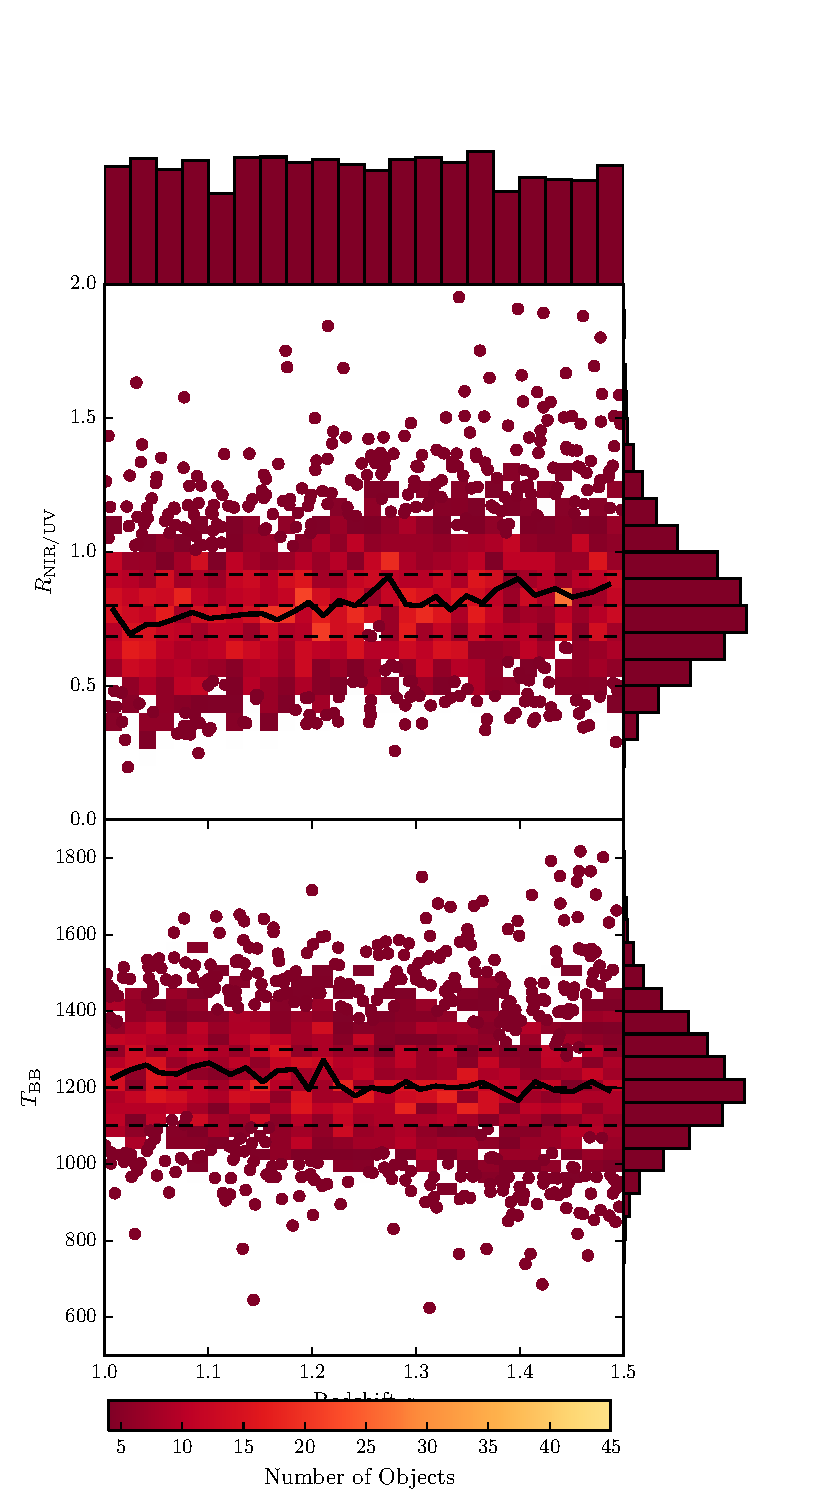
\includegraphics[width=0.8\textwidth]{figures/chapter06/ratio_bbt_z.pdf}
  \caption{Plot of $R_{{\rm NIR}/{\rm UV}}$ and $T_{BB}$ versus redshift. $L_{UV}$ defined as being lumionsity between 2000 and 10000A. $L_{IR}$ is lumionsity of blackbody component integrated everywhere. When we have more than 4 objects per grid cell we switch to using a density plot. Both $R_{{\rm NIR}/{\rm UV}}$ and $T_{BB}$ are approximately independent of redshift, with possible variations at $z > 1.2$.}
  \label{fig:}
\end{figure}

\begin{figure}
  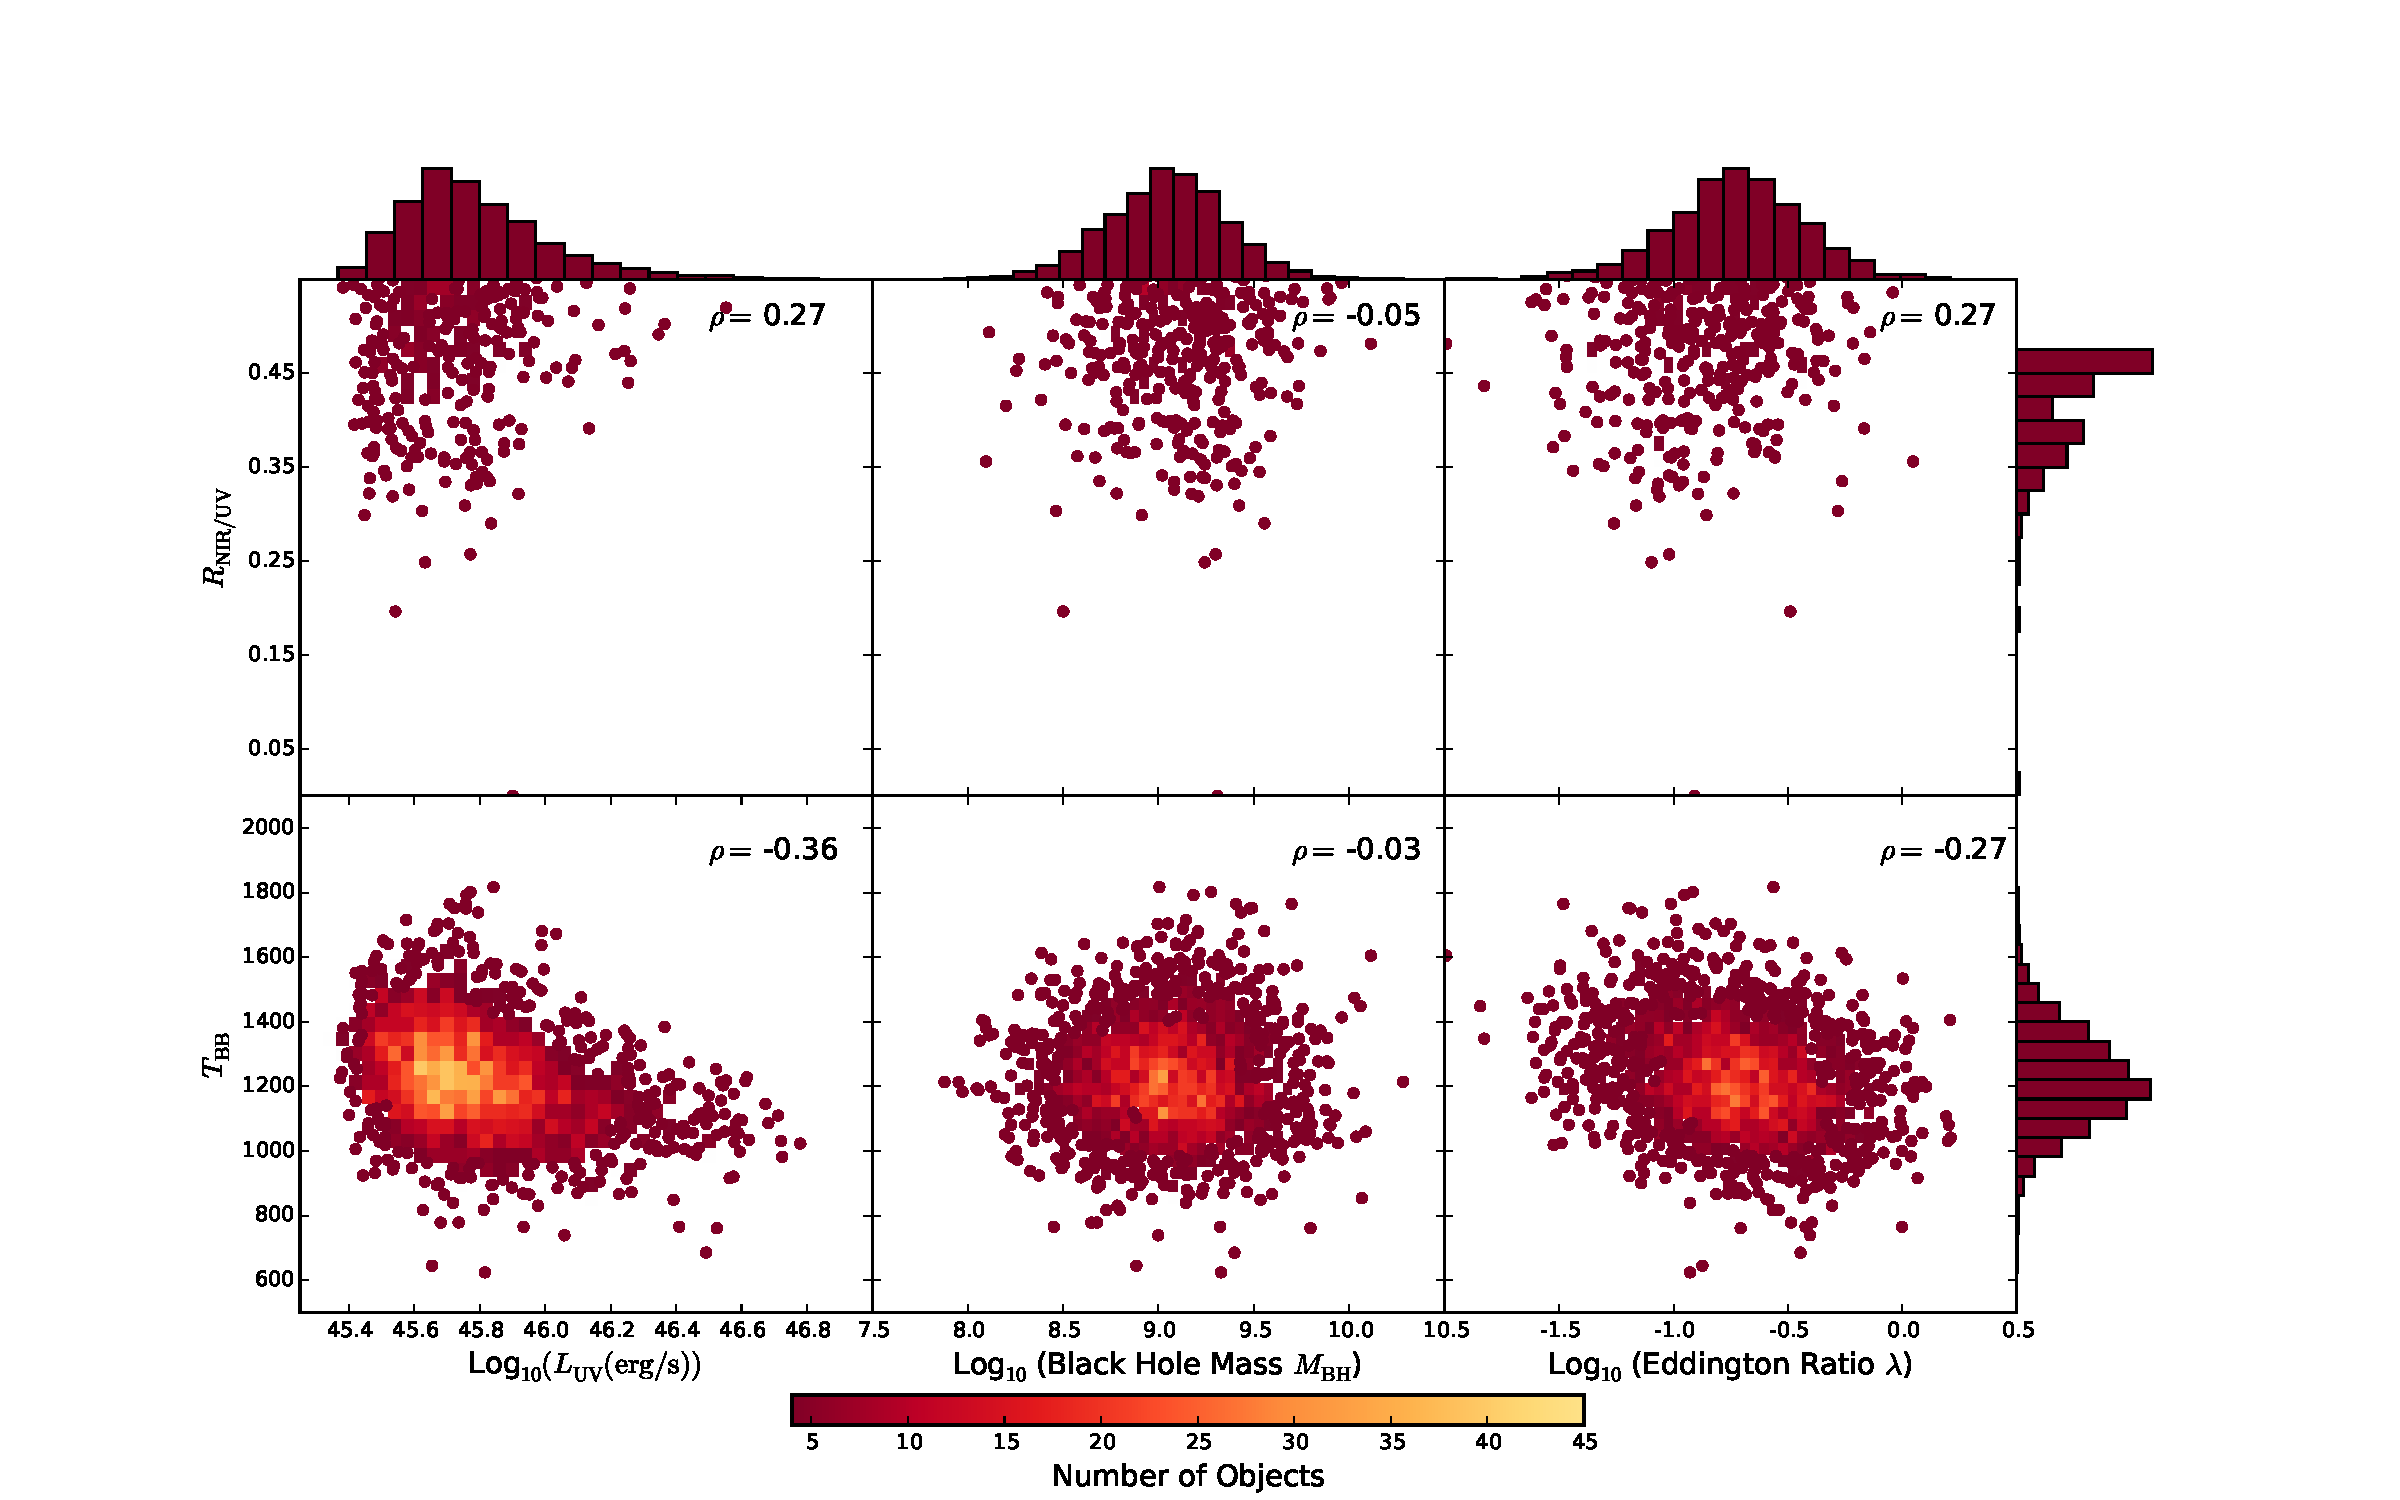
\includegraphics[width=\columnwidth]{figures/chapter06/correlations.pdf}
   \caption{Colour-bar might not be be accurate for each subfigure. CIV blueshift also positively correlated with Eddington Ratio.}
\end{figure}

We nowl look for correlations between the properties of the black-bodies we have fitted to the hot dust emission and other properties of the quasar such as redshift, black-hole mass, and normalised accretion rate (Eddington ratio). 

Firstly, we test whether the properties of the black-body evolve with redshift. In the Figure in the proceding section we plotted the temperature of the black-body component of our model as a function of redshift. This reveals evidence for a weak anti-correlation between the black-body temperature and the redshift ($\rho =$ -$0.09$, $p = 2e$-$10$). It could be that this apparent trend is an artifact of the fitting procedure. Although we constrained the redshift range of the sample specifically to mitigate for such an effect, the region of the rest-frame spectrum being fit is changing systematically as a function of redshift. To test this we fit a mock data set of SEDs with fixed black-body properties at a range of redshifts. The best-fit black-body temperatures are shown with the dashed black line in the Figure. There is no evidence for any change as a function of redshift. Furthermore, we showed in an above Figure that there is no evidence for any systematic change in the quality of the fit with redshift. It is also unlikely 

Of course, redshift and luminosity will always be correlated for a flux-limited sample such as this. Therefore we will now look for correlations of between the black-body temperature and luminosity, as well as the black-hole mass and Eddington ratio.

\section{Results From Blackbody Fit}

We fixed the overall normalisation of the quasar SEDs to values from the 2000 - 9000 \AA~ fit, and fit for the temperature and normalisation of the blackbody component in the 10,000 - 24,000 \AA~ region of the rest frame spectrum (i.e. the spectral region most sensitive to hot dust emission). 

\subsection{Results 1: $\beta_{\mathrm{NIR}}$, $T_{\mathrm{BB}}$, $R_{\mathrm{UV}/\mathrm{NIR}}$}

\begin{figure}
\centering
  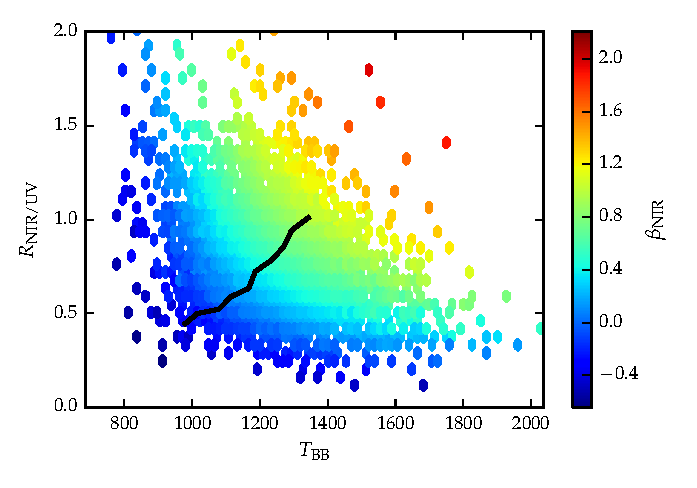
\includegraphics[width=\columnwidth]{figures/chapter06/ratio_tbb_beta.pdf}
  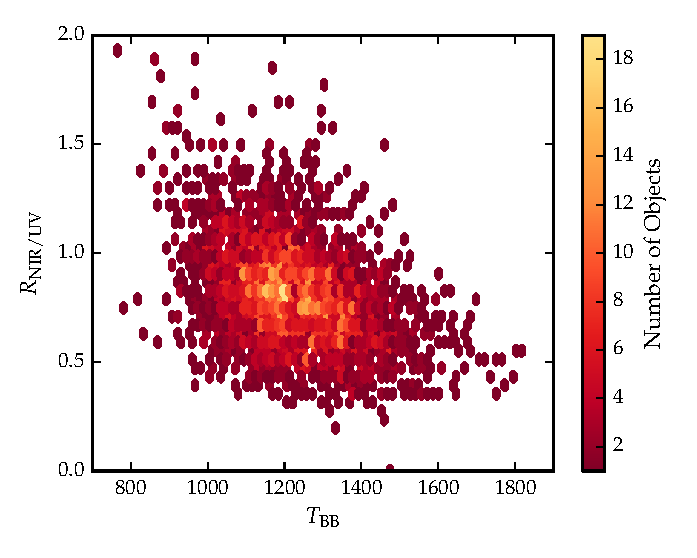
\includegraphics[width=\columnwidth]{figures/chapter06/ratio_tbb_beta_density.pdf}
\caption{ Plot of the near-IR/ultra violet luminosity ratio ($R_{\mathrm{NIR}/\mathrm{UV}}$) against the NIR power-law slope for the low-$z$ sample. The NIR lumionsity is measured by integrating the best-fit model spectrum (with a black body component) in the rest-frame of the quasar between 0.2 and 1 $\mu$m. The NIR power-law slope is fit between 1 and 2.4$\mu$m (although the exact wavelength region being fit depends on the redshift of the quasar; see somewhere else). This allows us to extend our investigation to high-$z$, where we are unable to constrain both the temperature and normalisation of the black-body component, but can constrain the slope of a single power-law. Included the second plot ecause I want to emphasise that the density of points is not constant - i.e. if you measure a certain value for beta, say 0.6, it's much more likely to be around (1200,0.2) than it is, say, (1100,0.3). Must be some way of quantifying this. I think there are different versions of this plot where LNIR has been calculated in different ways, so the y-axis is different. This uses lumcalc\_v3. }
  \label{fig:fig}
\end{figure}


Even with $T=1600K$, contribution from blackbody to UV luminosity only $\simeq 1\%$. 

\subsection{Results 2: Redshift}

\begin{figure}
\centering
  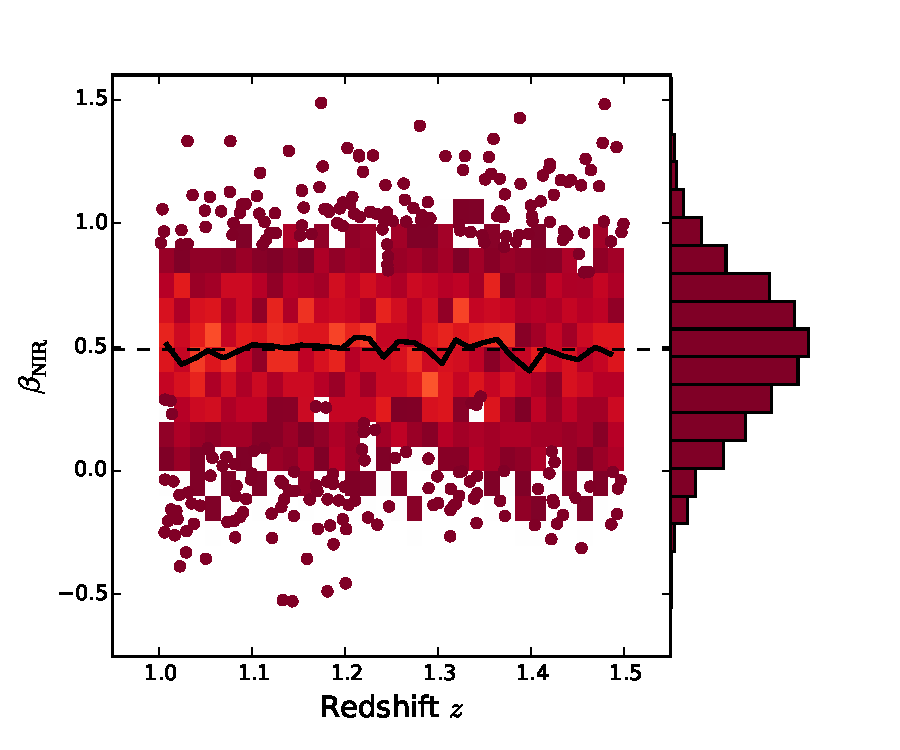
\includegraphics[width=\columnwidth]{figures/chapter06/beta_z_v1}
\caption{fgh}
  \label{fig:fig}
\end{figure}

\subsection{Results 3: Luminosity}

No correlation between $\beta$ (or $R_{{\rm UV}/{\rm NIR}}$) and $L_{\rm UV}$ (or any other measure of bolometric luminosity) but negative correlation with blackbody temperature. 

\subsection{Results 4: Eddington Ratio/ Black Hole Mass}

\begin{figure}
  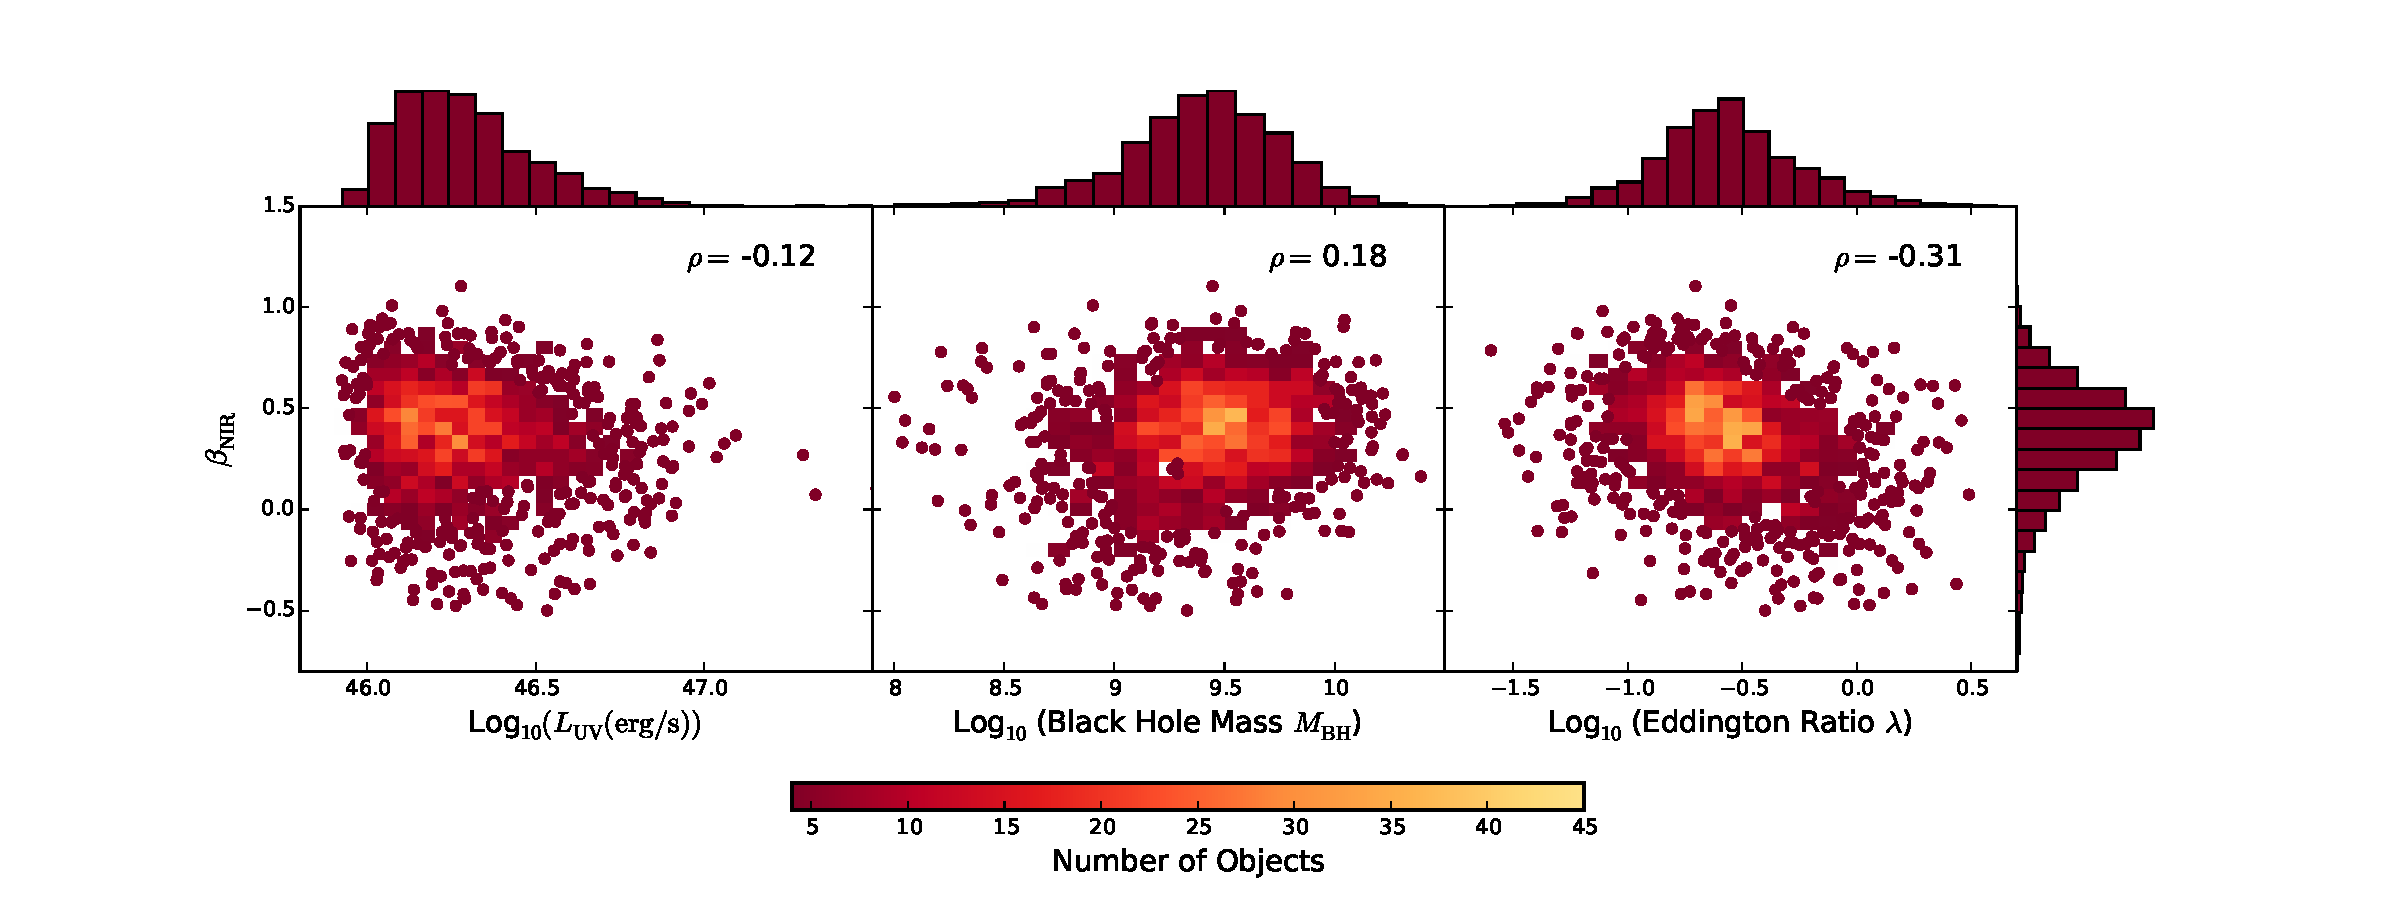
\includegraphics[width=\textwidth]{figures/chapter06/correlations_highz}
   \caption{IR/UV lumiosity ratio versus black hole mass (Shen et al.) for high-$z$ sample. Fairly strong negative correlation. We believe that this is just a manifestation of the fact that at high redshift the blackhole masses are derived from CIV. We already know that the FWHM of CIV has a positive correlation with the hot dust abundance, and large CIV FWHM leads to larger black hole mass estimates. This explains the apparent correlation between the IR/UV ratio and the black hole mass. Eddington ratio measures the luminosity relative to the Eddington luminosity. Higher blackhole mass estimates will lead to lower Eddington ratios, which is why the Eddington ratio appears to decrease with increaseing IR/UV ratio.}
\end{figure}

\subsection{C\,IV Emission Line Properties}

\begin{figure}
\centering
  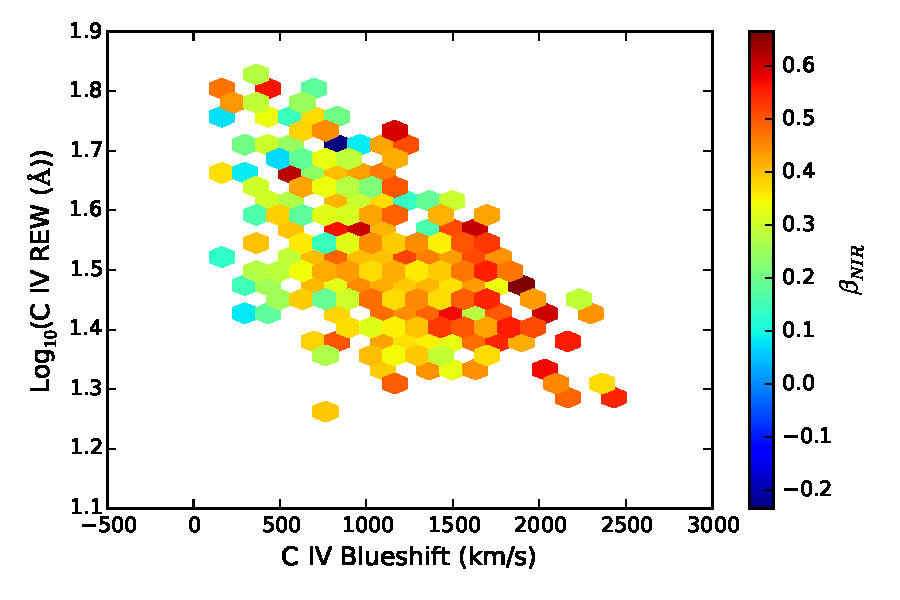
\includegraphics[width=\columnwidth]{figures/chapter06/civ_2d}
\caption{Now using same high-redshift sample as Figure 8 (with cut on beta uncertainty). I'm only plotting where I have a miniumum of two objects per bin, which is probably not acceptable. Clear non-virial component to CIV line - caveat about CIV based black hole masses. }
  \label{fig:fig}
\end{figure}



\subsection{Reddening}

\begin{figure}
\centering
  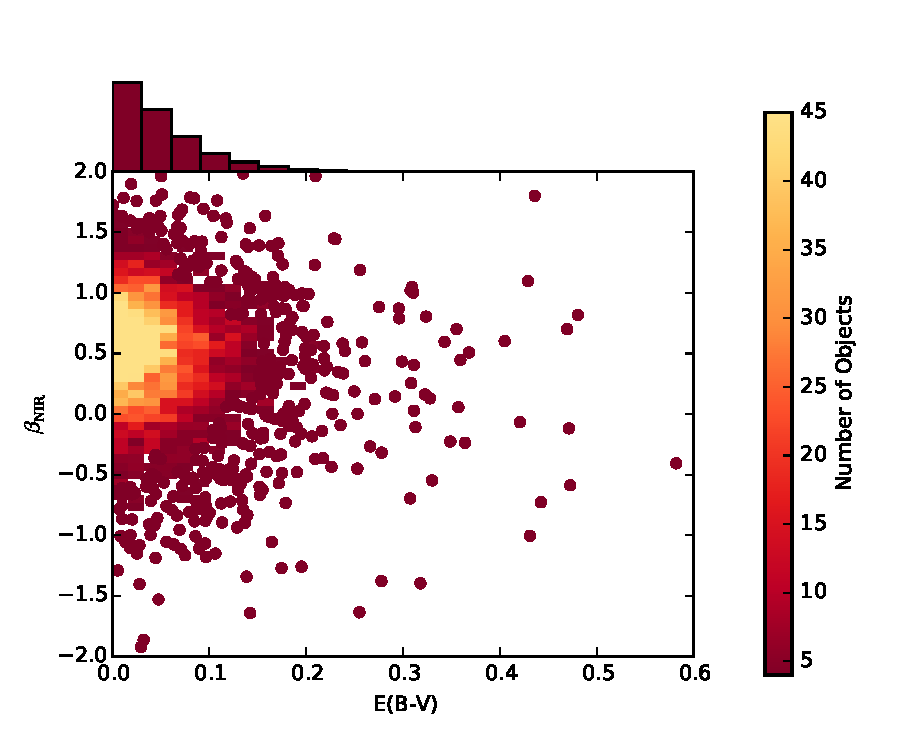
\includegraphics[width=\columnwidth]{figures/chapter06/ebv_beta}
\caption{Plot E(B-V) versus $\beta$. Just fit E(B-V) $<$ 1 micron and z $>$ 1 to avoid galaxy contribution. No cuts made to sample. No correlation/weak negative. I've got loads of plots like this. Some show positive correlation, some so negative, so I'm not sure what's going on.}
  \label{fig:fig}
\end{figure}

\subsection{BALs}

\begin{figure}
\centering
  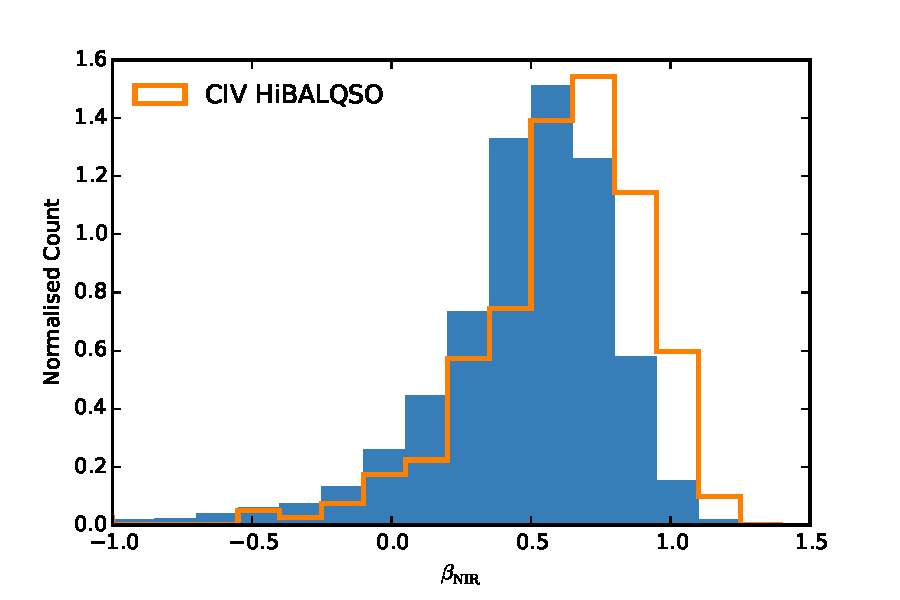
\includegraphics[width=\columnwidth]{figures/chapter06/BALs_hist}
\caption{High-$z$ only since very few BALs in low-$z$ sample. $\beta$ on $x$-axis. BALs clearly have bigger NIR slopes, so I would expect to also see $\beta$ increase with E(B-V), which I don't.}
  \label{fig:fig}
\end{figure}

At the same time, blue-shifted broad absorption troughs, associated with quasar-driven outflowing gas, are observed in about 20\% of quasars. 
At low-$z$, don't have sufficient numbers for reliable BAL/non-BAL comparison. At high-$z$ BALs appear to redder ($\beta=0.54$) than non-BALs ($\beta=0.43$). 

\subsection{RL/RQ}

\begin{figure}
\centering
  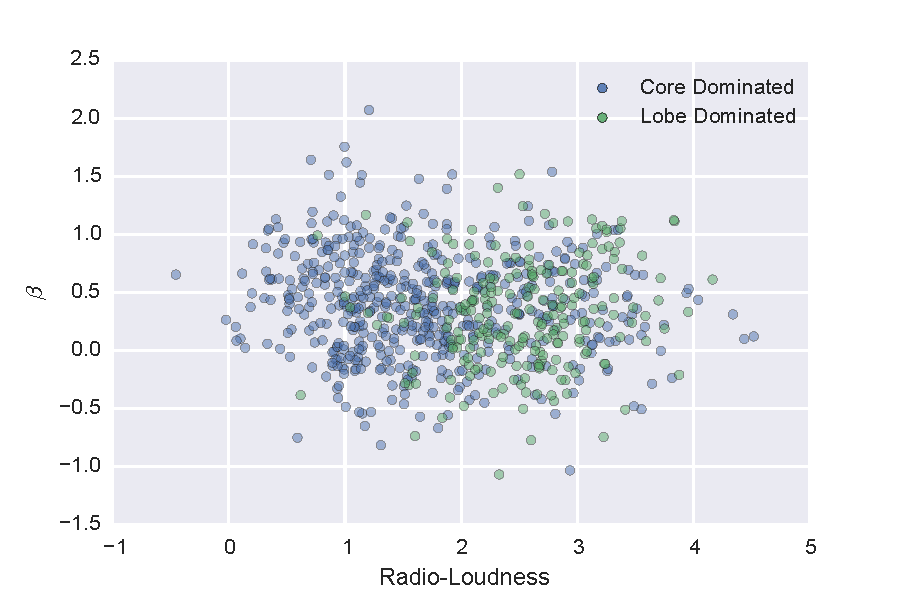
\includegraphics[width=\columnwidth]{figures/chapter06/radioloudness_beta}
\caption{Weak negative correlation for core-dominated sources and weak positive correlation for lobe-dominated sources.}
  \label{fig:fig}
\end{figure}

\begin{figure}
\centering
  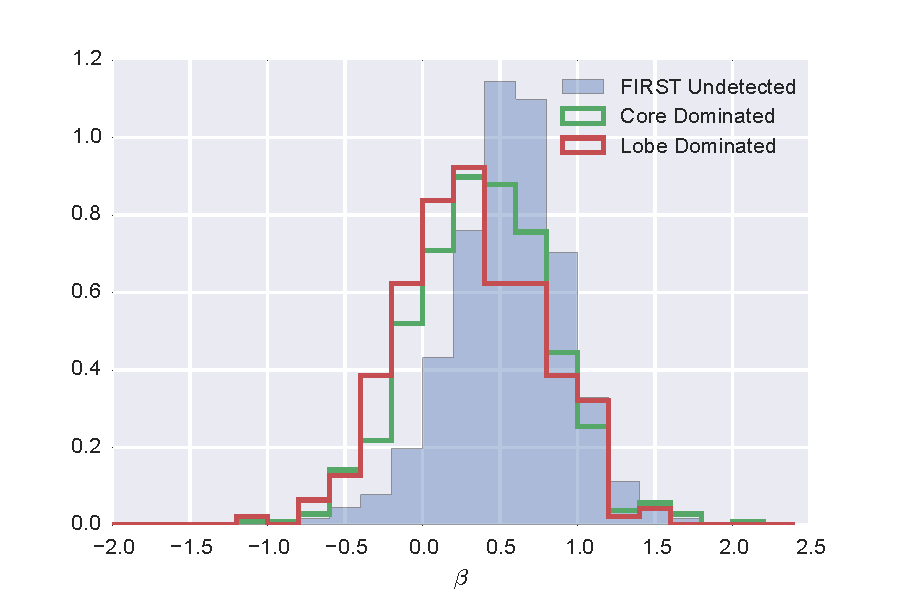
\includegraphics[width=\columnwidth]{figures/chapter06/radiohist}
\caption{Radio-loud objects appear to have less hot dust on average.  Statistically at least, the "radio-loud" objects are thought to have high black-hole masses and there is some form of radio-mode feedback (jet related) which is very different from the much more common (almost certainly wider opening-angle) outflow objects with large CIV-blueshifts.}
  \label{fig:fig}
\end{figure}


\begin{figure}
\centering
  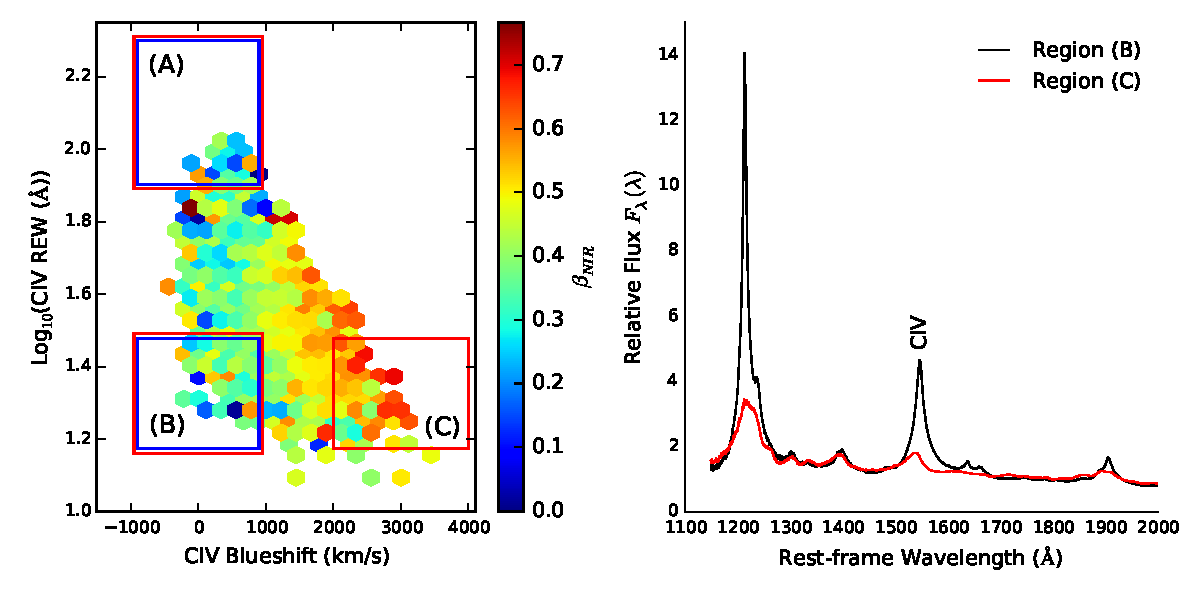
\includegraphics[width=\columnwidth]{figures/chapter06/ntt_proposal_figure1.pdf}
\caption{USE PLOT FROM RESEARCH PROPOSAL. Rest-frame equivalent width and blueshift of the \ion{C}{4} line for 7,115 SDSS DR7 quasars. The colours of the hexagons denote the median hot dust (T$\simeq$1200\,K) abundance for all
quasars at a given equivalent width and blueshift. The hot dust abundance is parameterised by fitting a single power-law with slope $\beta_{\mathrm NIR}$ beyond 1\,$\mu$m in the quasar rest-frame. Quasars with the most extreme outflow signatures (in region C) are predominantly hot-dust rich. The \ion{C}{4} emission line blueshift is obtained from the wavelength of the centroid of the emission line relative to the predicted location for emission at the systemic velocity of each quasar. Systemic redshifts are obtained from Hewett and Wild (2010).}
  \label{fig:}
\end{figure}


\begin{figure}
\centering
  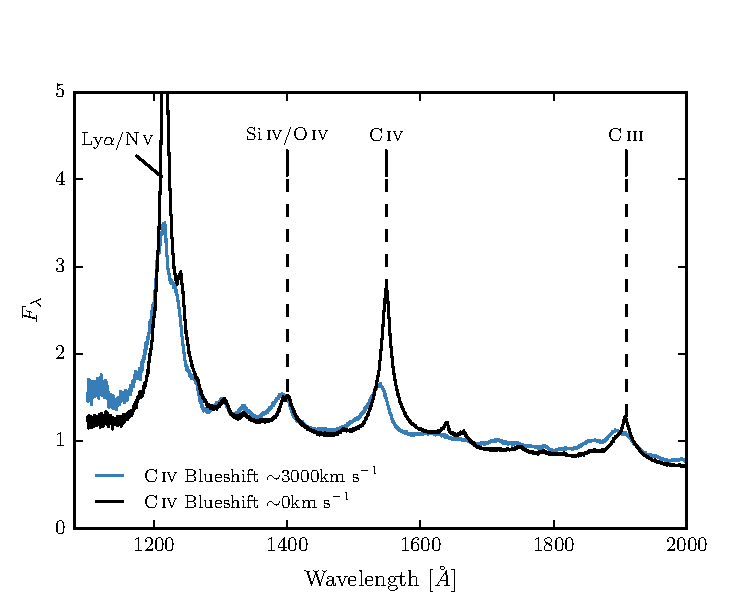
\includegraphics[width=\columnwidth]{figures/chapter06/blueshift_composite.pdf}
\caption{}
  \label{fig:}
\end{figure}

\begin{figure}
\centering
  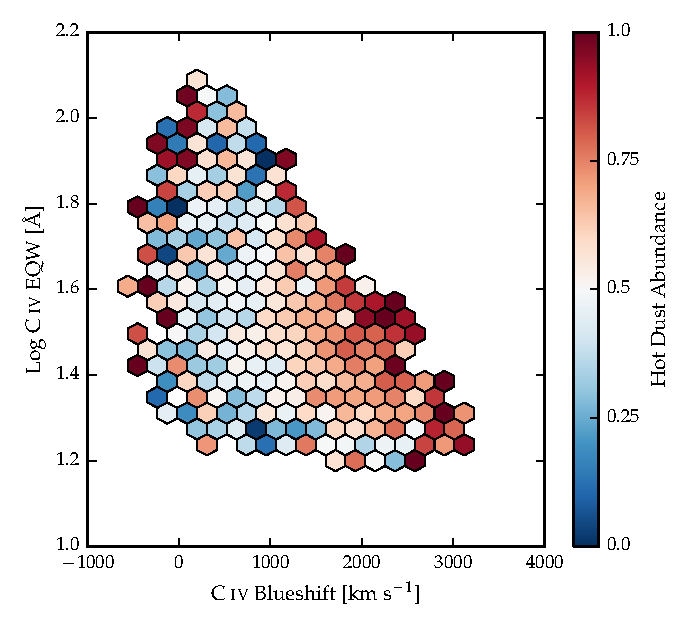
\includegraphics[width=\columnwidth]{figures/chapter06/hot_dust_beta.pdf}
\caption{}
  \label{fig:}
\end{figure}



\begin{figure}
\centering
  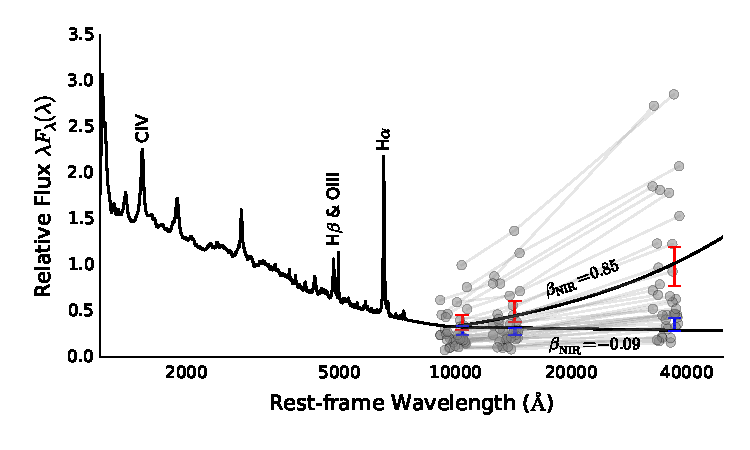
\includegraphics[width=\columnwidth]{figures/chapter06/ntt_proposal_figure2.pdf}
\caption{Representative rest-frame model spectra for the most hot-dust rich and hot-dust poor quasars in our SDSS sample, with error bars indicating the range of {\it WISE} W1, W2, and W3 magnitudes for the objects in these subsamples, transformed to the rest frame of the quasar. Grey lines show the W1, W2, and W3 fluxes for our sample of highly reddened quasars.}
  \label{fig:}
\end{figure}

There is a clear anti-correlation between the UV luminosity and the best-fit black-body temperature. We calculated a Spearman rank-order correlation coefficient -0.33. The fact that the blackbody temperature is anti-correlated with the luminosity could explain the weak anti-correlation between black-body temperature and redshift we saw in the Figure above. 

The black-hole masses are virial estimates calculated by Shen et al. 2011 using the MgII emission line in the SDSS spectra. There is no evidence for a correlation between the best-fit black-body temperature and the black-hole mass ($\rho=$-$0.02$, $p=0.15$).  

The Eddington ratios (bolometric luminosity normalised by Eddington luminosity) are also calculated by Shen et al. 2011 using bolometric corrections in Richards et al. (2006a) using 3000A monochromatic luminosities. There is a clear anti-correlation between the best-fit black-body temperature and the Eddington ratio ($\rho=$-0.25, $p=2.4e$-64). Given what we know about the trends of black-body temperature with luminosity and black-hole mass, this is to be expected. Eddington ratio is proportional to luminosity, which is anti-correlated with black-body temperature, and inversely proportional to the black-hole mass, which has no correlation with black-body temperature. Therefore it is to be expected that black-body temperature is anti-correlated with the Eddington ratio. 

Next, we look for correlations of some of the fundamental properties of quasars with the ratio of NIR to UV luminosity. In the previous section we showed a possible anti-correlation between the black-body temperature and the UV luminosity. As we discussed in an earlier section, the luminosity of hot dust is correlated with the temperature, such that lower-temperature hot dust has a greater luminosity. We emphasise this point in the Figure below, where we plot the ratio of NIR to UV luminosity against the black-body temperature, colour-coding the points by the UV luminosity. The UV luminosity changes most strongly as a function of temperature, but there is also a much weaker correlation with the NIR to UV luminosity ratio. We calculated a partial Spearman rank correlation coefficent of 0.10 after the mutual dependence of the NIR to UV luminosity ratio and the UV luminosity on temperature had been factored out. Another way of showing this is to take slices of constant temperature; this is shown in the Figure below. There is a very weak correlation, although it is not clear whether it is statistically significant. Note that by restricting the redshift range we are limiting the dynamic range in luminosity, which may be why we don't see the stronger trend observed by Roseboom et al. 




\section{Future Work}

This work will be built on by, for example, investigating dust-extinction (combining our sample with moderately-reddened quasars from Maddox et al. 2012 and heavily-reddened quasars from Banerji et al. 2012-2015), broad-absorption line quasars, and/or radio properties. We will also investigate the sub-population of quasars for which we don't observe any emission from hot dust. 









It is now well established that non-spherical geometries including some form of obscuring material/torus on parsec scales, can explain much of the observed diversity seen in the spectral energy distributions (SEDs) of AGN. 

Photometry from the \textit{WISE} satellite now provides information about the properties of the hot, dusty obscuring medium in the most luminous AGN. 
With information on the rest-frame SEDs covering rest-frame 0.1-3.0\,$\mu$m wavelengths for thousands of AGN
at redshifts $z$=2-3 it is finally possible to study the link between outflow diagnostics from ultraviolet spectra, e.g. as measured from the CIV emission line, and emission from hot dust, which provides information about the amount and geometry of gas and dust on parsec scales. 
In one model, quasars are surrounded by an inner `wall' of gas and dust, in a cylinder-like geometry. 
As a radiatively-driven outflow develops, material at the extremes of the cylinder is driven-off, exposing more of the inner edge of the obscuring material at the equator (a `torus'), which contains the hot dust. 

In Figure \ref{fig:w1w2colors} we plot the $W1 - W2$ colors of the DR7Q-matched sample as a function of redshift from $z=0.2$ to $z=1.8$. 
In this redshift range the $W1$ and $W2$ band-passes are probing the 12,000 - 28,000 \AA~ and 16,000 - 38,000 \AA~ region of the rest frame SED respectively, and the $W1-W2$ color is therefore predominantly tracing emission from hot dust at temperatures $\sim 1200$ K. At any given redshift or, equivalently, region of the rest-frame SED, we see a $\sim 0.5$ mag dispersion in the $W1-W2$ colors. On the same axes in Figure \ref{fig:w1w2colors} we have plotted the $W1 - W2$ colors derived from our SED model with blackbody temperatures ranging from 1000 - 1600 K and blackbody normalisation factors (i.e. the flux from the blackbody component relative to the power-law continuum at a reference wavelength) from 0 - 0.5, with the other parameters as reported in Table \ref{tab:params}. A blackbody with a single temperature and normalisation is clearly not a very good representation of the hot dust properties of the whole sample. For example, dust which is futher from the accretion disc will be at a lower temperature, and if the covering factor of the dust around the accretion disc is smaller then the ratio of near-IR luminosity to UV/optical luminosity (which the blackbody normalisation is proportional to) will decrease. We aim to study the diversity hot dust properties of the quasars in our sample to learn about the nature of the hot dust, and to link the hot dust properties to other physical quantities such as the luminosity and redshift of the quasar. 

\subsection{Defining Sample}
\label{sec:definingsample}

We decided to explore the diversity of hot dust properties by fitting our standard model, with the blackbody temperature and normalisation as free paramters, to the individual quasar SEDs. The first step was to define a sample of quasars from the DR7Q-matched catalogue which were well fit by our standard un-reddened SED model. To achieve this we discarded from our sample quasars with $i - K$ colors redder than our standard model with dust reddening E(B-V) = 0.1 (see Figure \ref{fig:ikvz}). As we discussed in Section \ref{sec:redobjects}, this region of the $i-K$ colour space includes both quasars with significant amounts of dust redenning and quasars with extreme emission line equivalent widths. We exclude quasars with observed magnitudes fainter than 19.1 in the $i$ band-pass, as well as quasars with upper-limit or S/R $<$ 5 magnitudes in the $K$, $W1$ and $W2$ band-passes (without these we will be unable to properly constrain the blackbody slope). We exclude quasars flagged as BALQSOs from the sample, since these objects may be in a special evolutionary stage and have different hot dust properties (we will consider this in future work). Finally, from all of the objects which passed the above criteria, we discarded the 10\% of quasars which were least well fit by our standard model.   

It is important to consider the redshift range over which we can reasonably expect to be able to constrain the shape of the blackbody component. The amount by which the observed spectrum is redshifted determines the position of the hot dust feature in the spectrum relative to the wavelength coverage of our set of band-passes. For a redshift $z \sim 1.5$ quasar, only the $W2$ band-pass, at $\sim 2 \mu$m in the rest frame of the quasar, is probing the wavelength region dominated by the blackbody emission (the peak in a $T \sim 1200$K blackbody is at $\sim 2.4 \mu$m). At $z \gtrsim 1.5$, we found that we could no longer constrain the shape of the blackbody component in our SED model using the $ugrizYJHKW1W2$ band-passes. Although we could include magnitude constraints from the longer-wavelength WISE $W3$ band-pass ($\lambda_{\rm eff} \simeq 12 \mu$m), at $z \sim 1.5$ this is observing $\sim 5 \mu$m in the quasar's rest frame. In this region there will be extra contributions to the flux, possibly from cooler dust, which are not accounted for in our model. This was clearly demonstrated by the increase in the $m_{\rm model} - m_{\rm data}$ residuals beyond $\sim 3\mu$m in the rest frame. At lower redshifts, the $W3$ band-pass is probing even longer-wavelengths, where the component we are missing from our model will be greater. To compensate our SED model will move the blackbody component to lower temperatures, which shifts the peak to longer wavelengths. The result will be a downward trend in the blackbody temperature with decreasing redshift. Given that one question we are interested in addressing is variations in the hot dust properties with redshift, we have to be very wary of systematic effects such as these. With these considerations in mind, we restricted ourselves to determining the hot dust properties of our quasar sample in the redshift range $0.5 < z < 1.5$. 

 

\section{Results From Blackbody Fit}

We fixed the overall normalisation of the quasar SEDs to values from the 2000 - 9000 \AA~ fit, and fit for the temperature and normalisation of the blackbody component in the 10,000 - 23,000 \AA~ region of the rest frame spectrum (i.e. the spectral region most sensitive to hot dust emission). In Figure \ref{fig:bbtvz} we show the best-fitting blackbody temperature for the quasars in our sample as a function of redshift. The solid lines are running-medians through the points, calculated both before and after we applied the correction to the model described in the preceding section. The difference is stark; after we apply the flux correction the median best-fitting blackbody temperature drops by $\sim 200$K to $\sim 1200$K. This is encouraging, since 1200K is the best-fitting blackbody temperature from the fit to the whole DR7Q-matched sample. Although we see no significant evolution of the hot dust properties in this redshift range, we plan to test this at higher redshift. We will also compare the hot dust properties of interesting subpopulations (e.g. Type II quasars, BALQSOs) and look for correlations with physical parameters of the quasar (e.g. luminosity, Eddington ratio). 

\begin{figure}
  \centering
  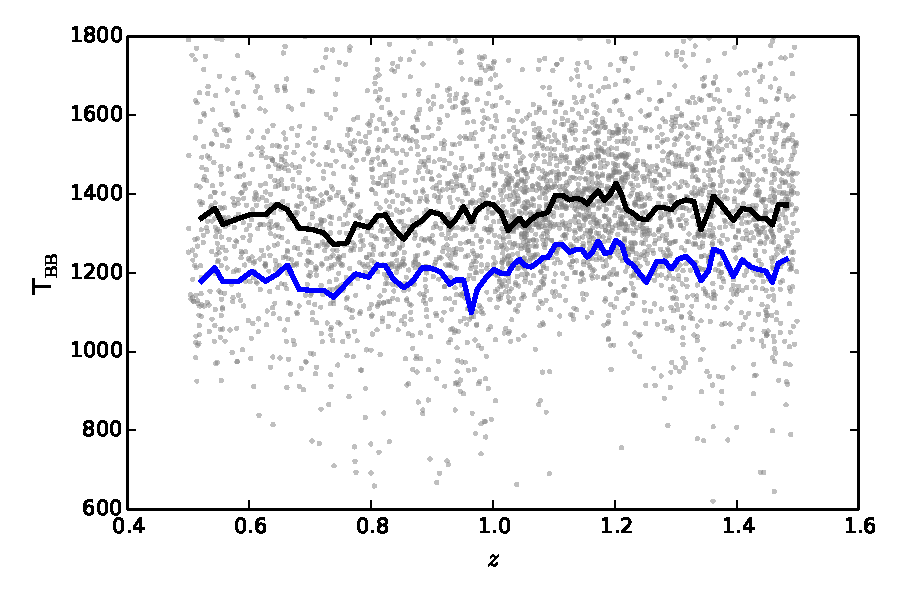
\includegraphics[width=\textwidth]{figures/chapter06/bbt_z.pdf}
  \caption{Blackbody temperature from fit against redshift before correction ({\it grey circles}). Black line is running median through blackbody temperatures before correction, blue line is running median after correction.}
  \label{fig:bbtvz}
\end{figure}

\newpage

\section{Conclusions and Future Work}

While many authors have focused on studies of specific sub-sets of AGN with extreme observational properties, what is missing is an understanding of how these extreme subsets relate to the population as a whole. In particular, we will focus on merger-based scenarios for quasar/galaxy co-evolution, which predict an obscured growth phase before the enshrouding dust is blown out, and schemes which explain the variety of observational properties as being only apparent differences due to non-spherical source geometries. We will study this issue by combining large-area photometric surveys from SDSS, UKIDSS and WISE. Multi-wavelength surveys allow us to gain a more holistic view of quasar properties by sampling their entire SED. We have a developed a model to fit the quasar SED in the 1 - 3 $\mu$m spectral region which, at present, can constrain the following features:

\begin{itemize}
\item {\bf Power-law slope}, which relates to properties of the accretion disk.
\item {\bf Blackbody temperature and normalisation}, which relates to properties of circum-nuclear hot dust. 
\item {\bf Dust Reddening}, at redshift of quasar, which relates to dust properties of the quasar and its host galaxy. 
\item {\bf Emission line strength}, which relates to properties of emission line regions and absorbing dust. 
\end{itemize}

The SDSS DR10Q catalogue, which was made available in late 2013, contains $\sim 120,000$ quasars at $z\gtrsim2$ ($\sim$ 5 times the number previously known). This will allow us to study quasar properties at the epoch when quasar activity peaked. Crucially, moderate-resolution optical spectra are available for all sources in the SDSS catalogue, which will allow us to relate SED properties to, for example, the black-hole mass and properties of outflowing gas. There is also the possibility, at least for a sub-set of objects, of extending our multi-wavelength SED coverage using data from, for example, FIRST in the radio and Spitzer in the far-IR. 

\subsubsection{Specific Investigations}

\subsubsection{Hot Dust Properties}

The near-IR excess in the SED is believed by many to be emission from dust at its sublimation temperature at the inner edge of a torus structure. We are able to test this by linking properties of the hot dust (e.g. the luminosity) to other properties of the quasar (e.g. bolometric luminosity, redshift). For example, is there any evidence for the inner edge of the torus being further from the nucleus in more luminous quasars (i.e. a decrease in near-IR to optical/UV luminosity ratio with increasing optical/UV luminosity)? Are there quasars in our sample which are deficient in hot dust and, if so, are these objects being observed before a dusty torus has formed or are the torus and accretion disk misaligned? 

\subsubsection{E(B-V) Distribution}

Deriving the dust-reddening E(B-V) distribution of our optically selected sample will allow us to relate the small samples of extremely reddened objects which have been found to the population of mildly reddened quasars. Are these extreme objects in the tail of a population of mildly reddened quasars or are there equal distributions of mildly reddened and extremely reddened quasars? A similar analysis was done by \citet{richards03}, but with the DR10Q catalogue we are able to pick up far more objects during the peak epoch when both quasar activity and star-formation rates peaked ($2 \lesssim z \lesssim 4$). Obtaining near-IR spectra for a sample of moderately reddened quasars will give us crucial information about the level and scale of the dust extinction. We will also use our sample to derive a new extinction curve appropriate for the quasar population.

\subsubsection{BALQSOs}

Broad, blue-shifted absorption lines are associated with AGN-driven out-flowing gas, and outflows are a key component in galaxy evolution models with AGN feedback. With an adapted model, we will derive information from the SED (e.g. the dust-reddening) which, when combined with outflow properties measured in the SDSS spectra, will allow us to study the population of BALQSOs in relation to the population as a whole. Are BALQSOs observed during a special `blow-out' phase in a quasars lifetime, or is outflowing gas only detected along certain sight-lines? 

\subsubsection{Type II Quasars}

How are the population of obscured Type II quasars related to the Type I population? Does the Seyfert Type I/II dusty-torus unification scheme extend to higher luminosities or are Type II quasars observed in a special phase of quasar growth? Again, properties derived from the multi-wavelength SEDs and optical spectra will help to relate these objects to the population as a whole. 




